\documentclass{article}
\usepackage{graphicx} % Required for inserting images
\usepackage{booktabs} % For better table rules
\usepackage{longtable} % For tables spanning multiple pages if necessary
\usepackage{float}
\usepackage{algorithm}
\usepackage{algorithmic}
\usepackage{amsmath}

\graphicspath{{./images/}}

\title{Programming Problem 1}
\author{Group 19 - Bertone and Hostic}
\date{November 2024}

\begin{document}

\maketitle

\section*{Problem Description}
We consider the Minimum Weighted Crossings with Constraints Problem (MWCCP), which is a generalization of the Minimum Crossings Problem. In the MWCCP we are given an undirected weighted bipartite graph \( G = (U \cup V, E) \) with node sets \( U = \{1, \dots, m\} \) and \( V = \{m + 1, \dots, n\} \) corresponding to the two partitions, edge set \( E \), and a set of constraints \( C \). The node sets \( U \) and \( V \) are disjoint. The edges \( e = (u, v) \in E \subseteq U \times V \) have associated weights \( w_e = w_{u,v} \). Precedence constraints \( C \) are given in the form of a set of ordered node pairs \( C \subseteq V \times V \), where \( (v, v') \in C \) means that node \( v \) must appear before node \( v' \) in a feasible solution.

The nodes of the graph \( G \) are to be arranged in two layers. The first layer contains all nodes of set \( U \) in fixed label order \( 1, \dots, m \), while the second layer contains the nodes of set \( V \) in an order to be determined. The goal of the MWCCP is to find an ordering of the nodes in \( V \) such that the weighted edge crossings are minimized while satisfying all constraints \( C \).

A candidate solution is thus represented by a permutation \( \pi = (\pi_{m+1}, \dots, \pi_n) \) of the nodes in \( V \). It is only feasible if all of the constraints \( C \) are fulfilled, i.e., \( \text{pos}_\pi(v) < \text{pos}_\pi(v') \), \( \forall (v, v') \in C \), where \( \text{pos}(v) \) refers to the position of a node \( v \in V \) in the permutation \( \pi \).

The objective function to be minimized is:
\[
f(\pi) = \sum_{(u, v) \in E} \sum_{\substack{(u', v') \in E \\ u < u'}} 
(w_{u,v} + w_{u', v'}) \cdot \delta_{\pi}((u, v), (u', v'))
\]
where
\[
\delta_{\pi}((u, v), (u', v')) = 
\begin{cases} 
1 & \text{if } \text{pos}_{\pi}(v) > \text{pos}_{\pi}(v'), \\ 
0 & \text{otherwise.} 
\end{cases}
\]

\section*{Question 1}
Application: Railway Scheduling and Track Layout
\begin{itemize}
    \item Nodes in \(U\) could represent fixed train stations along a route, where trains must stop in a specific order
    \item Nodes in \(V\) could represent trains/train routes to be scheduled within the network
    \item Weighted edges would indicate the relationship between trains/train routes and tracks, with higher weights representing either higher traffic, longer distance, lower importance in terms of scheduling (in case of for example local vs. high speed train)
    \item Constraints in C would enforce rules like the fact that certain trains need to arrive before others or that trains using the same tracks do not overlap.
\end{itemize}

The objective then would be to arrange the schedules in V to minimize the crossings of tracks while satisfying all constraints in C. This would lead to improved security and efficiency as minimizing track crossings would reduce the likelihood of collisions or delays due to track conflicts.


\section*{Q2: Deterministic Construction Heuristic}

\subsection*{Algorithm Description}

A meaningful deterministic construction heuristic could be one based on a greedy approach:
\begin{itemize}
    \item Initialize an empty ordered permutation list $\pi$ for nodes in $V$
    \item Compute for each node in $V$ the number of constraints that require other nodes to come before it
    \item Create a list of candidates with nodes in $V$ that have no predecessors
    \item For every node in the candidates and until $V$ is empty
    \begin{itemize}
        \item calculate the total weight of edges connecting it to U
        \item select the node with the lowest total edge weight to nodes in $U$ and append it to the final permutation list $\pi$
        \item  update the in-degree of nodes that had this as a constraint reducing it by $1$
        \item if the in-degree of any node in $V$ reaches zero add it to the candidates
        
    \end{itemize}
\end{itemize}

\subsection*{Components}

\paragraph{Input Structure:}
\begin{itemize}
    \item The graph structure includes nodes \( U \) and \( V \), edges \( E \), and edge weights.
    \item \textbf{Constraints:} A mapping of precedence relationships such that if \( v_1 \to v_2 \), node \( v_1 \) must precede \( v_2 \) in the final ordering.
\end{itemize}

\paragraph{Node Weight Precomputation:}
To imporve efficiency, the algorithm precomputes the sum of incoming edge weights for each node in \( V \). This will serve as a heuristic for selecting the "best" candidate node during construction.

\paragraph{Initialization of Candidates:}
Nodes with an in-degree of zero (i.e., no unfulfilled constraints) are initialized as candidates for the ordering. These nodes are stored in a \texttt{deque} for efficient addition and removal.

\paragraph{Greedy Node Selection:}
At each step, the algorithm selects the node from the candidates with the smallest total incoming edge weight. This \textbf{problem-specific heuristic} aims to minimize high-cost crossings early in the construction process.

\paragraph{Update Mechanism:}
Once a node is selected, it is removed from the candidate set and appended to the ordering \( \pi \). The algorithm then reduces the in-degrees of its dependent nodes. If a dependent node's in-degree becomes zero, it is added to the candidate set.

\paragraph{Solution Verification:}
After constructing \( \pi \), the algorithm verifies:
\begin{itemize}
    \item All nodes in \( V \) are included exactly once.
    \item All precedence constraints are respected
\end{itemize}

\subsection*{Adaptations}
\begin{itemize}
    \item \textbf{Problem-Specific Heuristic:} The algorithm prioritizes nodes with lower edge weights to reduce crossings early in the construction.
    \item \textbf{Constraint Management:} Using in-degrees to dynamically track feasible candidates ensures constraints are respected throughout the process.
    \item \textbf{Solution Verification:} A final verification step guarantees correctness.
\end{itemize}

\subsection*{Results}
The quality of the solution given by our Deterministic Construction Heuristic is competitive as it is visible from the competition results, while being very fast. Below we report some performance metrics for the different test instance sizes. The computations are performed using the free CPU for Colab (Intel Xeon CPU with 2 vCPUs) and 13GB of RAM.

\subsubsection*{Small}
\begin{table}[H]
\centering
\begin{tabular}{lcc}
\toprule
\textbf{Instance}         & \textbf{Time (s)} & \textbf{Cost} \\ 
\midrule
inst\_50\_4\_00002 & 0.000799 & 31619.0 \\ 
inst\_50\_4\_00004 & 0.000259 & 8582.0  \\ 
inst\_50\_4\_00007 & 0.000155 & 3463.0  \\ 
inst\_50\_4\_00005 & 0.000122 & 6034.0  \\ 
inst\_50\_4\_00009 & 0.000128 & 2633.0  \\ 
inst\_50\_4\_00003 & 0.000148 & 15511.0 \\ 
inst\_50\_4\_00006 & 0.000166 & 4883.0  \\ 
inst\_50\_4\_00010 & 0.000119 & 1658.0  \\ 
inst\_50\_4\_00001 & 0.000279 & 84883.0 \\ 
inst\_50\_4\_00008 & 0.000426 & 3005.0  \\ 
\bottomrule
\end{tabular}
\caption{Results for Small instances}
\end{table}

\subsubsection*{Medium}

\begin{table}[H]
\centering
\begin{tabular}{lcc}
\toprule
\textbf{Instance}         & \textbf{Time (s)} & \textbf{Cost} \\ 
\midrule
inst\_200\_20\_00008 & 0.000852 & 709644.0   \\ 
inst\_200\_20\_00001 & 0.001486 & 23033165.0 \\ 
inst\_200\_20\_00009 & 0.000805 & 547596.0   \\ 
inst\_200\_20\_00010 & 0.000881 & 461537.0   \\ 
inst\_200\_20\_00006 & 0.000879 & 1217519.0  \\ 
inst\_200\_20\_00004 & 0.000938 & 2551528.0  \\ 
inst\_200\_20\_00005 & 0.001722 & 1627621.0  \\ 
inst\_200\_20\_00003 & 0.001898 & 4361007.0  \\ 
inst\_200\_20\_00007 & 0.001528 & 908103.0   \\ 
inst\_200\_20\_00002 & 0.002308 & 8390614.0  \\ 
\bottomrule
\end{tabular}
\caption{Results for Medium instances}
\end{table}

\subsubsection*{Medium-Large}
\begin{table}[H]
\centering
\begin{tabular}{lcc}
\toprule
\textbf{Instance}         & \textbf{Time (s)} & \textbf{Cost} \\ 
\midrule
inst\_500\_40\_00001 & 0.012615 & 40802322.0  \\ 
inst\_500\_40\_00010 & 0.021615 & 247294126.0 \\ 
inst\_500\_40\_00019 & 0.015958 & 532473137.0 \\ 
inst\_500\_40\_00013 & 0.012978 & 334007118.0 \\ 
inst\_500\_40\_00007 & 0.016719 & 168022855.0 \\ 
inst\_500\_40\_00016 & 0.015179 & 437097158.0 \\ 
inst\_500\_40\_00004 & 0.009197 & 94454966.0  \\ 
\bottomrule
\end{tabular}
\caption{Results for Medium-Large instances}
\end{table}


\subsubsection*{Large}
\begin{table}[H]
\centering
\begin{tabular}{lcc}
\toprule
\textbf{Instance}         & \textbf{Time (s)} & \textbf{Cost} \\ 
\midrule
inst\_1000\_60\_00005 & 0.032712 & 1065285851.0  \\ 
inst\_1000\_60\_00002 & 0.066785 & 5340801153.0  \\ 
inst\_1000\_60\_00004 & 0.039137 & 1614552426.0  \\ 
inst\_1000\_60\_00001 & 0.136459 & 15151194763.0 \\ 
inst\_1000\_60\_00003 & 0.045279 & 2701197831.0  \\ 
inst\_1000\_60\_00007 & 0.027055 & 569249713.0   \\ 
inst\_1000\_60\_00006 & 0.030169 & 767270792.0   \\ 
inst\_1000\_60\_00008 & 0.039558 & 451262171.0   \\ 
inst\_1000\_60\_00009 & 0.027395 & 358976591.0   \\ 
inst\_1000\_60\_00010 & 0.031849 & 293146116.0   \\ 
\bottomrule
\end{tabular}
\caption{Results for Large instances}
\end{table}





\section*{Q3: Randomized Construction Heuristic}
The randomized heuristic could roughly follow the same process as the deterministic one, but then, when choosing the node in $V$ to add to the final permutation list $\pi$, instead of always choosing the one that has a minimum weighted sum of edges to $U$, pick one randomly, with a probability inversely proportional to this sum.
In particular we will use a Boltzmann Distribution to balance randomness and greedy choice. 

\paragraph{Probability Calculation:}
Compute the probabilities for selecting a node from the current candidates using a Boltzmann distribution. More in details:
\begin{itemize}
    \item Calculate scores for all candidate nodes
    \item Normalize the scores to avoid overflow
    \item Compute the probabilities using: 
    \(p_i = \frac{\exp{(-\frac{s_i}{\alpha})}}{\sum_j \exp{(-\frac{s_j}{\alpha})}}\), where \(s_i\) is the normalized score for node \( i\).
\end{itemize}
The parameter $\alpha$ controls randomness: a smaller $\alpha$ increases randomness, while a larger value value favors greediness.
In this way, nodes with higher cost/score have lower probability to be selected.

\paragraph{Single Solution Construction:}
The steps are very similar to the deterministic construction heuristic.
\begin{itemize}
    \item Start with all nodes having in-degree zero.
    \item Randomly select a node from candidates using the probabilities.
    \item Add the node to the ordering, remove it from the candidates, and update in-degrees of connected nodes.
    \item Repeat until all nodes are ordered.
\end{itemize}


\paragraph{Multiple Iterations:}
We also add the possibility to run the single-solution construction multiple times to improve the results and get lower variance. In particular the steps are:
\begin{itemize}
    \item Repeat the construction process $num_iterations$ times.
    \item Evaluate the cost of each solution.
    \item Keep the best solution found.
\end{itemize}


\subsection*{Results}
The results are computed using a single iteration and a parameter $\alpha = 0.6$. The randomized construction is repeated 30 times and the results are averaged. The computations are performed using the free CPU for Colab (Intel Xeon CPU with 2 vCPUs) and 13GB of RAM.

\subsubsection*{Small}


\begin{table}[H]
\centering
\hspace*{-1.5cm}
\begin{tabular}{llllll}
\toprule
\textbf{Item} & \textbf{Avg Time (s)} & \textbf{Avg Cost} & \textbf{Min Cost} & \textbf{Max Cost} & \textbf{Std Dev} \\
\midrule
\texttt{inst\_50\_4\_00002} & 0.003626 & 30855.97 & 27857.00 & 32643.00 & 1050.59 \\
\texttt{inst\_50\_4\_00004} & 0.003219 & 9172.10  & 7928.00  & 10239.00 & 500.92  \\
\texttt{inst\_50\_4\_00007} & 0.001821 & 3578.43  & 2827.00  & 4096.00  & 288.79  \\
\texttt{inst\_50\_4\_00005} & 0.002545 & 5569.87  & 4853.00  & 6219.00  & 351.73  \\
\texttt{inst\_50\_4\_00009} & 0.002607 & 2492.43  & 2091.00  & 2784.00  & 191.61  \\
\texttt{inst\_50\_4\_00003} & 0.003283 & 15485.43 & 13478.00 & 16528.00 & 722.92  \\
\texttt{inst\_50\_4\_00006} & 0.002801 & 4650.20  & 4092.00  & 5232.00  & 290.86  \\
\texttt{inst\_50\_4\_00010} & 0.001948 & 1620.17  & 1355.00  & 1975.00  & 131.56  \\
\texttt{inst\_50\_4\_00001} & 0.003809 & 84930.00 & 80297.00 & 88682.00 & 2078.92 \\
\texttt{inst\_50\_4\_00008} & 0.001744 & 2915.70  & 2136.00  & 3360.00  & 273.16  \\
\midrule
\textbf{Summary Statistics} & \textbf{0.002740} & \textbf{16127.03} & - & - & - \\
\bottomrule
\end{tabular}
\label{tab:performance_metrics_randomized}
\end{table}

\subsubsection*{Medium}
\begin{table}[H]
\centering
\hspace*{-1.5cm}
\begin{tabular}{llllll}
\toprule
\textbf{Item} & \textbf{Avg Time (s)} & \textbf{Avg Cost} & \textbf{Min Cost} & \textbf{Max Cost} & \textbf{Std Dev} \\
\midrule
\texttt{inst\_200\_20\_00010} & 0.015873 & 456531.27  & 445306.00   & 470534.00   & 7330.93   \\
\texttt{inst\_200\_20\_00009} & 0.015896 & 543713.67  & 521951.00   & 568060.00   & 11855.02  \\
\texttt{inst\_200\_20\_00006} & 0.019273 & 1207213.20 & 1166898.00  & 1238370.00  & 18112.10  \\
\texttt{inst\_200\_20\_00003} & 0.029675 & 4327121.80 & 4250721.00  & 4399702.00  & 42645.01  \\
\texttt{inst\_200\_20\_00002} & 0.043474 & 8361784.40 & 8195701.00  & 8506730.00  & 82622.20  \\
\texttt{inst\_200\_20\_00004} & 0.037687 & 2551007.27 & 2490237.00  & 2615850.00  & 30495.64  \\
\texttt{inst\_200\_20\_00007} & 0.030310 & 904974.73  & 881311.00   & 939154.00   & 15387.23  \\
\texttt{inst\_200\_20\_00001} & 0.061063 & 23195717.50 & 22931228.00 & 23599133.00 & 162599.73 \\
\texttt{inst\_200\_20\_00008} & 0.016568 & 713576.87  & 679658.00   & 739042.00   & 15210.27  \\
\texttt{inst\_200\_20\_00005} & 0.021958 & 1613500.70 & 1561975.00  & 1656848.00  & 23931.89  \\
\midrule
\textbf{Summary Statistics} & \textbf{0.029178} & \textbf{4387514.14} & - & - & - \\
\bottomrule
\end{tabular}
\label{tab:medium_performance_metrics_randomized}
\end{table}

\subsubsection*{Medium-Large}
\begin{table}[H]
\centering
\hspace*{-2cm}
\begin{tabular}{llllll}
\toprule
\textbf{Item} & \textbf{Avg Time (s)} & \textbf{Avg Cost} & \textbf{Min Cost} & \textbf{Max Cost} & \textbf{Std Dev} \\
\midrule
\texttt{inst\_500\_40\_00001} & 0.177799 & 41306375.60  & 40921403.00  & 41835187.00  & 249191.77  \\
\texttt{inst\_500\_40\_00010} & 0.396382 & 248177497.60 & 246238999.00 & 249837668.00 & 920296.47  \\
\texttt{inst\_500\_40\_00019} & 0.603033 & 533048783.97 & 528410832.00 & 536610229.00 & 2055959.77 \\
\texttt{inst\_500\_40\_00013} & 0.450295 & 334334851.00 & 332129824.00 & 336682608.00 & 1098089.99 \\
\texttt{inst\_500\_40\_00007} & 0.342089 & 167237198.67 & 165989443.00 & 168598596.00 & 719070.85  \\
\texttt{inst\_500\_40\_00016} & 0.535916 & 436747201.67 & 433165807.00 & 439570395.00 & 1724318.23 \\
\texttt{inst\_500\_40\_00004} & 0.261199 & 94402713.37  & 92471418.00  & 95619239.00  & 828955.05  \\
\midrule
\textbf{Summary Statistics} & \textbf{0.395245} & \textbf{265036374.55} & - & - & - \\
\bottomrule
\end{tabular}
\label{tab:medium_large_performance_metrics_randomized}
\end{table}

\subsubsection*{Large}

\begin{table}[H]
\centering
\hspace*{-2cm}
\begin{tabular}{llllll}
\toprule
\textbf{Item} & \textbf{Avg Time (s)} & \textbf{Avg Cost} & \textbf{Min Cost} & \textbf{Max Cost} & \textbf{Std Dev} \\
\midrule
\texttt{inst\_1000\_60\_00005} & 1.940377 & 1067764674.70  & 1060835463.00  & 1075136067.00  & 3443214.33  \\
\texttt{inst\_1000\_60\_00002} & 5.258952 & 5339427349.17  & 5316206983.00  & 5358163297.00  & 9952612.22  \\
\texttt{inst\_1000\_60\_00004} & 2.576052 & 1618919043.03  & 1604354503.00  & 1629522719.00  & 5881501.28  \\
\texttt{inst\_1000\_60\_00001} & 9.653994 & 15145125818.07 & 15119309857.00 & 15174139010.00 & 15114903.03 \\
\texttt{inst\_1000\_60\_00003} & 3.577870 & 2710183271.13  & 2698638355.00  & 2723048821.00  & 6434495.93  \\
\texttt{inst\_1000\_60\_00007} & 1.234546 & 568833774.80   & 564743332.00   & 571513933.00   & 1777165.09  \\
\texttt{inst\_1000\_60\_00006} & 1.506673 & 771255574.13   & 765180918.00   & 777979955.00   & 3043546.59  \\
\texttt{inst\_1000\_60\_00008} & 1.053052 & 450177254.10   & 446090463.00   & 455253372.00   & 2137433.51  \\
\texttt{inst\_1000\_60\_00009} & 0.886946 & 357376938.03   & 354133103.00   & 359544918.00   & 1668191.08  \\
\texttt{inst\_1000\_60\_00010} & 0.773536 & 294319001.80   & 291894077.00   & 297714026.00   & 1198184.49  \\
\midrule
\textbf{Summary Statistics} & \textbf{2.846200} & \textbf{2832338269.90} & - & - & - \\
\bottomrule
\end{tabular}
\label{tab:large_performance_metrics_randomized}
\end{table}


\subsubsection*{Experimenting with number of repetitions}
We notice that if we increase the number of repetitions allowed the quality of the results starts increasing and becoming more stable.

\begin{table}[H]
    \centering
    \hspace*{-1.5cm}
    \begin{tabular}{lrrrrr}
        \toprule
        \textbf{Item} & \textbf{Avg Time (s)} & \textbf{Avg Cost} & \textbf{Min Cost} & \textbf{Max Cost} & \textbf{Std Dev} \\
        \midrule
        inst\_50\_4\_00005 & 0.002378 & 5345.13 & 4772.00 & 6478.00 & 380.12 \\
        inst\_50\_4\_00001 & 0.004306 & 85259.53 & 81247.00 & 90229.00 & 2232.76 \\
        inst\_50\_4\_00008 & 0.001885 & 2808.87 & 2116.00 & 3227.00 & 299.90 \\
        inst\_50\_4\_00003 & 0.003003 & 15488.67 & 13773.00 & 16915.00 & 717.22 \\
        inst\_50\_4\_00002 & 0.003352 & 29928.00 & 27555.00 & 31895.00 & 1162.61 \\
        inst\_50\_4\_00009 & 0.002575 & 2365.97 & 1946.00 & 2803.00 & 239.67 \\
        inst\_50\_4\_00004 & 0.003143 & 9307.63 & 8242.00 & 10415.00 & 532.04 \\
        inst\_50\_4\_00007 & 0.002303 & 3685.53 & 2877.00 & 4369.00 & 379.83 \\
        inst\_50\_4\_00010 & 0.002392 & 1601.17 & 1293.00 & 1946.00 & 172.61 \\
        inst\_50\_4\_00006 & 0.003085 & 4351.13 & 3771.00 & 5001.00 & 273.22 \\
        \midrule
        \multicolumn{6}{l}{\textbf{Summary Statistics:}} \\
        \multicolumn{6}{l}{Average time across all instances: 0.002842 seconds} \\
        \multicolumn{6}{l}{Average cost across all instances: 16014.16} \\
        \bottomrule
    \end{tabular}
\end{table}

\section*{Q4: Local Search}
We developed a framework for basic local search able to deal with different neighborhood structures and different step functions.

\subsection*{Local Search Procedure}

The local search algorithm follows these steps:

\begin{enumerate}
    \item \textbf{Initialization:} 
    \begin{itemize}
        \item Start with an initial solution \( \text{current\_solution} \).
        \item Set key parameters:
        \begin{itemize}
            \item Maximum number of iterations (\( \text{max\_iter} \)).
            \item Maximum plateau (\( \text{max\_plateau} \)), i.e., consecutive iterations without improvement before termination.
        \end{itemize}
    \end{itemize}
    
    \item \textbf{Neighborhood Generation:}
    \begin{itemize}
        \item Generate a set of neighboring solutions using a selected neighborhood structure among:
        \begin{itemize}
            \item Swap
            \item Window
            \item Block Shift
        \end{itemize}
    \end{itemize}
    
    \item \textbf{Solution Selection:}
    \begin{itemize}
        \item Select the next solution based on the chosen step function. Three different step functions are allowed:
        \begin{itemize}
            \item \textbf{Best Improvement:} Explore all neighbors and select the one with the lowest cost.
            \item \textbf{First Improvement:} Select the first neighbor that improves the current cost.
            \item \textbf{Random:} Select a random neighbor from the set of valid neighbors.
        \end{itemize}
    \end{itemize}
    
    \item \textbf{Iteration:}
    \begin{itemize}
        \item Evaluate the cost of the selected solution using the cost function \( f(\text{s}) \).
        \item Update the best solution and plateau counter:
        \begin{itemize}
            \item If the selected solution improves the best cost, update \( \text{best\_solution} \) and reset the plateau counter.
            \item Otherwise, increment the plateau counter.
        \end{itemize}
    \end{itemize}
    
    \item \textbf{Termination:}
    \begin{itemize}
        \item Stop the search when either:
        \begin{itemize}
            \item The maximum number of iterations (\( \text{max\_iter} \)) is reached.
            \item The plateau counter exceeds \( \text{max\_plateau} \).
        \end{itemize}
    \end{itemize}
    
    \item \textbf{Statistics:}
    \begin{itemize}
        \item Record statistics such as runtime.
    \end{itemize}
\end{enumerate}

\subsection*{Results}
The computations are performed using the free CPU for Colab (Intel Xeon CPU with 2 vCPUs) and 13GB of RAM.

\subsubsection*{Neighborhood: Swap - Step Function: Best Improvement}

\begin{table}[H]
\centering
\caption{Local Search Results for Small Instances ($max\_iterations = 50$)}
\begin{tabular}{lccc}
\toprule
\textbf{Instance} & \textbf{Best Cost} & \textbf{Runtime (s)} & \textbf{Iterations} \\
\midrule
inst\_50\_4\_00007 & 2,512.0  & 0.10 & 50 \\
inst\_50\_4\_00004 & 7,396.0  & 0.13 & 50 \\
inst\_50\_4\_00001 & 77,867.0 & 0.42 & 50 \\
inst\_50\_4\_00005 & 4,812.0  & 0.13 & 50 \\
inst\_50\_4\_00002 & 27,746.0 & 0.25 & 50 \\
inst\_50\_4\_00008 & 2,012.0  & 0.09 & 50 \\
inst\_50\_4\_00009 & 2,042.0  & 0.07 & 50 \\
inst\_50\_4\_00006 & 3,853.0  & 0.11 & 50 \\
inst\_50\_4\_00010 & 1,110.0  & 0.06 & 50 \\
inst\_50\_4\_00003 & 13,622.0 & 0.17 & 50 \\
\bottomrule
\end{tabular}
\label{tab:small_instance_results}
\end{table}

\begin{table}[H]
\centering
\caption{Local Search Results for Medium Instances ($max\_iterations = 50$)}
\begin{tabular}{lccc}
\toprule
\textbf{Instance} & \textbf{Best Cost} & \textbf{Runtime (s)} & \textbf{Iterations} \\
\midrule
inst\_200\_20\_00008 & 699,180.0    & 3.07  & 50 \\
inst\_200\_20\_00004 & 2,531,002.0  & 4.26  & 50 \\
inst\_200\_20\_00001 & 22,966,065.0 & 13.55 & 50 \\
inst\_200\_20\_00009 & 538,575.0    & 2.10  & 50 \\
inst\_200\_20\_00003 & 4,336,083.0  & 6.55  & 50 \\
inst\_200\_20\_00006 & 1,206,819.0  & 2.77  & 50 \\
inst\_200\_20\_00002 & 8,355,692.0  & 8.55  & 50 \\
inst\_200\_20\_00005 & 1,611,936.0  & 3.32  & 50 \\
inst\_200\_20\_00007 & 897,361.0    & 2.46  & 50 \\
inst\_200\_20\_00010 & 456,187.0    & 1.84  & 50 \\
\bottomrule
\end{tabular}
\label{tab:medium_instance_results}
\end{table}

\begin{table}[H]
\centering
\caption{Local Search Results for Medium-Large Instances ($max\_iterations = 50$)}
\begin{tabular}{lccc}
\toprule
\textbf{Instance} & \textbf{Best Cost} & \textbf{Runtime (s)} & \textbf{Iterations} \\
\midrule
inst\_500\_40\_00001 & 40,763,525.0   & 41.96  & 50 \\
inst\_500\_40\_00010 & 247,156,541.0  & 106.64 & 50 \\
inst\_500\_40\_00019 & 532,261,363.0  & 191.66 & 50 \\
inst\_500\_40\_00007 & 167,906,057.0  & 90.77  & 50 \\
inst\_500\_40\_00004 & 94,371,986.0   & 70.22  & 50 \\
inst\_500\_40\_00016 & 436,874,308.0  & 200.25 & 50 \\
inst\_500\_40\_00013 & 333,834,201.0  & 157.92 & 50 \\
\bottomrule
\end{tabular}
\label{tab:large_instance_results}
\end{table}

\begin{table}[H]
\centering
\caption{Local Search Results for Large Instances ($max\_iterations = 50$)}
\begin{tabular}{lccc}
\toprule
\textbf{Instance} & \textbf{Best Cost} & \textbf{Runtime (s)} & \textbf{Iterations} \\
\midrule
inst\_1000\_60\_00006 & 767,127,903.0  & 506.02  & 50 \\
inst\_1000\_60\_00005 & 1,065,098,886.0 & 560.25  & 50 \\
inst\_1000\_60\_00003 & 2,700,811,057.0 & 1032.99 & 50 \\
inst\_1000\_60\_00009 & 358,889,249.0   & 397.72  & 50 \\
inst\_1000\_60\_00002 & 5,340,320,884.0 & 1725.27 & 50 \\
inst\_1000\_60\_00010 & 293,073,569.0   & 361.81  & 50 \\
inst\_1000\_60\_00004 & 1,614,325,406.0   & 984.39  & 50 \\
inst\_1000\_60\_00008 & 451,158,389.0   & 491.05  & 50 \\
inst\_1000\_60\_00007 & 569,125,154.0   & 614.16  & 50 \\
inst\_1000\_60\_00001 & 15,150,318,365.0  & 2484.93 & 50 \\
\bottomrule
\end{tabular}
\label{tab:local_search_results}
\end{table}

\subsubsection*{Neighborhood: Swap - Step Function: First Improvement}

\begin{table}[H]
\centering
\caption{Local Search Results for Small Instances ($max\_iterations = 50$)}
\begin{tabular}{lccc}
\toprule
\textbf{Instance} & \textbf{Best Cost} & \textbf{Runtime (s)} & \textbf{Iterations} \\
\midrule
inst\_50\_4\_00007 & 2,706.0   & 0.19 & 50 \\
inst\_50\_4\_00004 & 7,579.0   & 0.26 & 50 \\
inst\_50\_4\_00001 & 81,263.0  & 0.66 & 50 \\
inst\_50\_4\_00005 & 5,317.0   & 0.19 & 50 \\
inst\_50\_4\_00002 & 29,552.0  & 0.40 & 50 \\
inst\_50\_4\_00008 & 2,609.0   & 0.14 & 50 \\
inst\_50\_4\_00009 & 2,070.0   & 0.19 & 50 \\
inst\_50\_4\_00006 & 4,496.0   & 0.13 & 50 \\
inst\_50\_4\_00010 & 1,232.0   & 0.15 & 50 \\
inst\_50\_4\_00003 & 14,276.0  & 0.28 & 50 \\
\bottomrule
\end{tabular}
\label{tab:local_search_results_50_4}
\end{table}

\begin{table}[H]
\centering
\caption{Local Search Results for Medium Instances ($max\_iterations = 50$)}
\begin{tabular}{lccc}
\toprule
\textbf{Instance} & \textbf{Best Cost} & \textbf{Runtime (s)} & \textbf{Iterations} \\
\midrule
inst\_200\_20\_00008 & 708,188.0   & 1.82 & 50 \\
inst\_200\_20\_00004 & 2,547,178.0 & 4.14 & 50 \\
inst\_200\_20\_00001 & 22,999,030.0 & 13.93 & 50 \\
inst\_200\_20\_00009 & 546,480.0   & 2.28 & 50 \\
inst\_200\_20\_00003 & 4,352,176.0 & 4.47 & 50 \\
inst\_200\_20\_00006 & 1,214,679.0 & 2.65 & 50 \\
inst\_200\_20\_00002 & 8,377,020.0 & 9.92 & 50 \\
inst\_200\_20\_00005 & 1,624,715.0 & 3.01 & 50 \\
inst\_200\_20\_00007 & 906,715.0   & 3.68 & 50 \\
inst\_200\_20\_00010 & 460,706.0   & 1.85 & 50 \\
\bottomrule
\end{tabular}
\label{tab:local_search_results_200_20}
\end{table}


\begin{table}[H]
\centering
\caption{Local Search Results for Medium-Large Instances ($max\_iterations = 50$)}
\begin{tabular}{lccc}
\toprule
\textbf{Instance} & \textbf{Best Cost} & \textbf{Runtime (s)} & \textbf{Iterations} \\
\midrule
inst\_500\_40\_00001 & 40,791,505.0  & 18.16 & 50 \\
inst\_500\_40\_00010 & 247,247,327.0 & 50.57 & 50 \\
inst\_500\_40\_00019 & 532,415,681.0 & 68.52 & 50 \\
inst\_500\_40\_00007 & 167,975,154.0 & 35.08 & 50 \\
inst\_500\_40\_00004 & 94,435,322.0  & 34.83 & 50 \\
inst\_500\_40\_00016 & 437,038,479.0 & 72.73 & 50 \\
inst\_500\_40\_00013 & 333,961,766.0 & 88.49 & 50 \\
\bottomrule
\end{tabular}
\label{tab:local_search_results_500_40}
\end{table}


\begin{table}[H]
\centering
\caption{Local Search Results for Large Instances ($max\_iterations = 50$)}
\begin{tabular}{lccc}
\toprule
\textbf{Instance} & \textbf{Best Cost} & \textbf{Runtime (s)} & \textbf{Iterations} \\
\midrule
inst\_1000\_60\_00006 & 767,238,025.0  & 109.37 &  50 \\
inst\_1000\_60\_00005 & 1,065,247,648.0 & 161.43 & 50 \\
inst\_1000\_60\_00003 & 2,701,111,013.0 & 168.95 & 50 \\
inst\_1000\_60\_00009 & 358,959,640.0   & 75.49  & 50 \\
inst\_1000\_60\_00002 & 5,340,602,179.0 & 252.40 & 50 \\
inst\_1000\_60\_00010 & 293,128,293.0   & 64.66  & 50 \\
inst\_1000\_60\_00004 & 1,614,471,356.0 & 129.18 & 50 \\
inst\_1000\_60\_00008 & 451,236,666.0   & 80.51  & 50 \\
inst\_1000\_60\_00007 & 569,234,502.0   & 93.38  & 50 \\
inst\_1000\_60\_00001 & 15,150,853,379.0 & 481.15 & 50 \\
\bottomrule
\end{tabular}

\label{tab:local_search_instances}
\end{table}

\subsubsection*{Neighborhood: Swap - Step Function: Random}
The max\_plateau is increased to 40 for small and medium instances and 30 for medium-large and large.

\begin{table}[H]
\centering
\caption{Average Local Search Results for Small Instances ($reps = 30$)}

\hspace*{-1cm}
\begin{tabular}{lccc}
\toprule
\textbf{Instance} & \textbf{Avg. Best Cost} & \textbf{Avg. Runtime (s)} & \textbf{Avg. Iterations} \\
\midrule
inst\_50\_4\_00007 & 3391.50  & 0.02  & 46.73 \\
inst\_50\_4\_00004 & 8486.53  & 0.03  & 48.13 \\
inst\_50\_4\_00001 & 84362.80 & 0.12  & 48.27 \\
inst\_50\_4\_00005 & 5953.67  & 0.02  & 47.53 \\
inst\_50\_4\_00002 & 31322.83 & 0.05  & 48.97 \\
inst\_50\_4\_00008 & 2910.63  & 0.02  & 48.73 \\
inst\_50\_4\_00009 & 2546.13  & 0.01  & 48.97 \\
inst\_50\_4\_00006 & 4809.47  & 0.02  & 48.40 \\
inst\_50\_4\_00010 & 1629.83  & 0.01  & 47.40 \\
inst\_50\_4\_00003 & 15332.03 & 0.04  & 48.07 \\
\bottomrule
\end{tabular}
\label{tab:average_results_50_4}
\end{table}

\begin{table}[H]
\centering
\caption{Average Local Search Results for Medium Instances ($reps = 20$)}
\hspace*{-1cm}
\begin{tabular}{lccc}
\toprule
\textbf{Instance} & \textbf{Avg. Best Cost} & \textbf{Avg. Runtime (s)} & \textbf{Avg. Iterations} \\
\midrule
inst\_200\_20\_00008 & 709057.10   & 0.28  & 48.15 \\
inst\_200\_20\_00004 & 2550888.75  & 0.55  & 46.15 \\
inst\_200\_20\_00001 & 23028645.15 & 1.82  & 48.35 \\
inst\_200\_20\_00009 & 547247.50   & 0.34  & 47.55 \\
inst\_200\_20\_00003 & 4359837.70  & 0.73  & 46.85 \\
inst\_200\_20\_00006 & 1217100.55  & 0.34  & 46.05 \\
inst\_200\_20\_00002 & 8389388.85  & 1.06  & 46.40 \\
inst\_200\_20\_00005 & 1626958.45  & 0.47  & 48.15 \\
inst\_200\_20\_00007 & 907582.55   & 0.31  & 48.40 \\
inst\_200\_20\_00010 & 461260.50   & 0.27  & 47.05 \\
\bottomrule
\end{tabular}
\label{tab:average_results_200_20}
\end{table}

\begin{table}[H]
\centering
\caption{Average Local Search Results for Medium-Large Instances ($reps=10$)}
\hspace*{-1cm}
\begin{tabular}{lccc}
\toprule
\textbf{Instance} & \textbf{Avg. Best Cost} & \textbf{Avg. Runtime (s)} & \textbf{Avg. Iterations} \\
\midrule
inst\_500\_40\_00001 & 40800240.60   & 3.50  & 43.20 \\
inst\_500\_40\_00010 & 247288200.30  & 7.48  & 41.60 \\
inst\_500\_40\_00019 & 532462011.60  & 10.69 & 42.40 \\
inst\_500\_40\_00007 & 168019163.30  & 5.92  & 39.60 \\
inst\_500\_40\_00004 & 94450515.90   & 4.97  & 43.30 \\
inst\_500\_40\_00016 & 437085267.70  & 10.35 & 44.90 \\
inst\_500\_40\_00013 & 333996882.40  & 9.09  & 45.40 \\
\bottomrule
\end{tabular}
\label{tab:average_results_500_40}
\end{table}

\begin{table}[ht]
\centering
\caption{Average Local Search Results for Large Instances ($reps=5$)}
\hspace*{-1cm}
\begin{tabular}{lccc}
\toprule
\textbf{Instance} & \textbf{Avg. Best Cost} & \textbf{Avg. Runtime (s)} & \textbf{Avg. Iterations} \\
\midrule
inst\_1000\_60\_00006 & 767258491.40   & 19.54  & 47.60 \\
inst\_1000\_60\_00005 & 1065284222.00  & 16.94  & 39.20 \\
inst\_1000\_60\_00003 & 2701180750.60  & 28.78  & 43.80 \\
inst\_1000\_60\_00009 & 358969702.20   & 12.59  & 46.40 \\
inst\_1000\_60\_00002 & 5340770534.00  & 41.02  & 45.40 \\
inst\_1000\_60\_00010 & 293142350.60   & 10.66  & 42.80 \\
inst\_1000\_60\_00004 & 1614536913.20  & 22.25  & 43.40 \\
inst\_1000\_60\_00008 & 451256811.20   & 13.99  & 46.60 \\
inst\_1000\_60\_00007 & 569244706.80   & 15.17  & 46.60 \\
inst\_1000\_60\_00001 & 15151148695.40 & 62.14  & 42.60 \\
\bottomrule
\end{tabular}
\label{tab:average_results_500_40}
\end{table}

\subsubsection*{Neighborhood: Window - Step Function: Best Improvement}

\begin{table}[H]
\centering
\caption{Results for Small Instances ($max\_iterations=50$, $window=3$)}
\begin{tabular}{lccc}
\toprule
\textbf{Instance} & \textbf{Best Cost} & \textbf{Runtime (s)} & \textbf{Iterations} \\
\midrule
inst\_50\_4\_00005 & 3973.0   & 2.05  & 50 \\
inst\_50\_4\_00001 & 74672.0  & 4.99  & 50 \\
inst\_50\_4\_00008 & 1536.0   & 0.99  & 50 \\
inst\_50\_4\_00003 & 12266.0  & 2.18  & 50 \\
inst\_50\_4\_00002 & 25003.0  & 4.34  & 50 \\
inst\_50\_4\_00009 & 1878.0   & 0.54  & 49 \\
inst\_50\_4\_00004 & 6576.0   & 1.68  & 50 \\
inst\_50\_4\_00007 & 2086.0   & 1.06  & 50 \\
inst\_50\_4\_00010 & 1053.0   & 0.51  & 50 \\
inst\_50\_4\_00006 & 3298.0   & 1.35  & 50 \\
\bottomrule
\end{tabular}
\label{tab:results_50_4}
\end{table}

\begin{table}[ht]
\centering
\caption{Results for Medium Instances ($max\_iterations=50$, $window=3$)}
\begin{tabular}{lccc}
\toprule
\textbf{Instance} & \textbf{Best Cost} & \textbf{Runtime (s)} & \textbf{Iterations} \\
\midrule
inst\_200\_20\_00009 & 531927.0   & 77.45  & 50 \\
inst\_200\_20\_00004 & 2511461.0  & 150.52 & 50 \\
inst\_200\_20\_00001 & 22902196.0 & 479.96 & 50 \\
inst\_200\_20\_00003 & 4316931.0  & 210.69 & 50 \\
inst\_200\_20\_00002 & 8321140.0  & 293.19 & 50 \\
inst\_200\_20\_00006 & 1198488.0  & 99.81  & 50 \\
inst\_200\_20\_00007 & 891163.0   & 87.67  & 50 \\
inst\_200\_20\_00010 & 451770.0   & 66.90  & 50 \\
inst\_200\_20\_00008 & 689139.0   & 83.05  & 50 \\
inst\_200\_20\_00005 & 1598406.0  & 119.89 & 50 \\
\bottomrule
\end{tabular}
\label{tab:results_200_20}
\end{table}

\begin{table}[H]
\centering
\caption{Results for Medium-Large Instances ($max\_iterations=25$, $window=3$)}
\begin{tabular}{lccc}
\toprule
\textbf{Instance} & \textbf{Best Cost} & \textbf{Runtime (s)} & \textbf{Iterations} \\
\midrule
inst\_500\_40\_00007 & 167915775.0  & 195.84 & 25 \\
inst\_500\_40\_00016 & 436859315.0  & 371.97 & 25 \\
inst\_500\_40\_00019 & 532268481.0  & 491.62 & 25 \\
inst\_500\_40\_00010 & 247149101.0  & 266.27 & 25 \\
inst\_500\_40\_00013 & 333836574.0  & 323.40 & 25 \\
inst\_500\_40\_00001 & 40762259.0   & 88.04  & 25 \\
inst\_500\_40\_00004 & 94369980.0   & 140.67 & 25 \\
\bottomrule
\end{tabular}
\label{tab:results_500_40}
\end{table}

\begin{table}[H]
\centering
\caption{Results for Large Instances ($max\_iterations=5$, $window=3$)}
\begin{tabular}{lccc}
\toprule
\textbf{Instance} & \textbf{Best Cost} & \textbf{Runtime (s)} & \textbf{Iterations} \\
\midrule
inst\_1000\_60\_00008 & 451237980.0   & 127.17 & 5 \\
inst\_1000\_60\_00001 & 15150997983.0 & 823.13 & 5 \\
inst\_1000\_60\_00003 & 2701109805.0  & 370.82 & 5 \\
inst\_1000\_60\_00002 & 5340694114.0  & 511.55 & 5 \\
inst\_1000\_60\_00009 & 358956889.0   & 129.90 & 5 \\
inst\_1000\_60\_00007 & 569221389.0   & 158.27 & 5 \\
inst\_1000\_60\_00006 & 767237776.0   & 209.52 & 5 \\
inst\_1000\_60\_00010 & 293128361.0   & 109.56 & 5 \\
inst\_1000\_60\_00005 & 1065241551.0  & 255.48 & 5 \\
inst\_1000\_60\_00004 & 1614500876.0  & 306.14 & 5 \\
\bottomrule
\end{tabular}
\label{tab:results_1000_60}
\end{table}


\subsubsection*{Neighborhood: Window - Step Function: First Improvement}

\begin{table}[H]
\centering
\caption{Results for Small Instances ($max\_iterations = 50$, $window=3$)}
\begin{tabular}{lccc}
\toprule
\textbf{Instance} & \textbf{Best Cost} & \textbf{Runtime (s)} & \textbf{Iterations} \\
\midrule
inst\_50\_4\_00005 & 5336.0   & 0.45  & 50 \\
inst\_50\_4\_00001 & 81525.0  & 1.56  & 50 \\
inst\_50\_4\_00008 & 2609.0   & 0.37  & 50 \\
inst\_50\_4\_00003 & 14341.0  & 0.56  & 50 \\
inst\_50\_4\_00002 & 29552.0  & 0.98  & 50 \\
inst\_50\_4\_00009 & 2187.0   & 0.56  & 50 \\
inst\_50\_4\_00004 & 7674.0   & 1.03  & 50 \\
inst\_50\_4\_00007 & 2935.0   & 0.77  & 50 \\
inst\_50\_4\_00010 & 1249.0   & 0.62  & 50 \\
inst\_50\_4\_00006 & 4499.0   & 0.32  & 50 \\
\bottomrule
\end{tabular}
\label{tab:results_50_4}
\end{table}

\begin{table}[H]
\centering
\caption{Results for Medium Instances ($max\_iterations = 50$, $window = 3$)}
\begin{tabular}{lccc}
\toprule
\textbf{Instance} & \textbf{Best Cost} & \textbf{Runtime (s)} & \textbf{Iterations} \\
\midrule
inst\_200\_20\_00009 & 546528.0   & 7.24  & 50 \\
inst\_200\_20\_00004 & 2547726.0  & 9.65  & 50 \\
inst\_200\_20\_00001 & 22999030.0 & 31.21 & 50 \\
inst\_200\_20\_00003 & 4352176.0  & 11.54 & 50 \\
inst\_200\_20\_00002 & 8377020.0  & 25.50 & 50 \\
inst\_200\_20\_00006 & 1214679.0  & 6.49  & 50 \\
inst\_200\_20\_00007 & 906997.0   & 7.24  & 50 \\
inst\_200\_20\_00010 & 461039.0   & 2.71  & 50 \\
inst\_200\_20\_00008 & 708188.0   & 5.45  & 50 \\
inst\_200\_20\_00005 & 1624715.0  & 7.43  & 50 \\
\bottomrule
\end{tabular}
\label{tab:results_200_20}
\end{table}

\begin{table}[H]
\centering
\caption{Results for Medium-Large Instances ($max\_iterations = 50$, $window=3$)}
\begin{tabular}{lccc}
\toprule
\textbf{Instance} & \textbf{Best Cost} & \textbf{Runtime (s)} & \textbf{Iterations} \\
\midrule
inst\_500\_40\_00007 & 167975154.0 & 80.89  & 50 \\
inst\_500\_40\_00016 & 437042675.0 & 166.65 & 50 \\
inst\_500\_40\_00019 & 532415681.0 & 158.86 & 50 \\
inst\_500\_40\_00010 & 247247327.0 & 120.93 & 50 \\
inst\_500\_40\_00013 & 333961766.0 & 235.75 & 50 \\
inst\_500\_40\_00001 & 40791505.0  & 45.80  & 50 \\
inst\_500\_40\_00004 & 94435322.0  & 81.53  & 50 \\
\bottomrule
\end{tabular}
\label{tab:results_500_40}
\end{table}

\begin{table}[H]
\centering
\caption{Results for Large Instances ($max\_iterations = 25$, $window = 3$)}
\begin{tabular}{lccc}
\toprule
\textbf{Instance} & \textbf{Best Cost} & \textbf{Runtime (s)} & \textbf{Iterations} \\
\midrule
inst\_1000\_60\_00008 & 451252292.0   & 65.93  & 25 \\
inst\_1000\_60\_00001 & 15151026458.0 & 489.53 & 25 \\
inst\_1000\_60\_00003 & 2701152697.0  & 136.62 & 25 \\
inst\_1000\_60\_00002 & 5340696178.0  & 200.09 & 25 \\
inst\_1000\_60\_00009 & 358968584.0   & 66.87  & 25 \\
inst\_1000\_60\_00007 & 569242224.0   & 89.64  & 25 \\
inst\_1000\_60\_00006 & 767257429.0   & 98.71  & 25 \\
inst\_1000\_60\_00010 & 293136774.0   & 43.63  & 25 \\
inst\_1000\_60\_00005 & 1065267951.0  & 145.68 & 25 \\
inst\_1000\_60\_00004 & 1614515234.0  & 100.29 & 25 \\
\bottomrule
\end{tabular}
\label{tab:results_1000_60}
\end{table}

\subsubsection*{Neighborhood: Window - Step Function: Random}
The max\_plateau variable is set to 30.

\begin{table}[H]
\centering
\caption{Average Results for Small Instances ($reps = 20$)}
\begin{tabular}{lccc}
\toprule
\textbf{Instance} & \textbf{Avg. Best Cost} & \textbf{Avg. Runtime (s)} & \textbf{Avg. Iterations} \\
\midrule
inst\_50\_4\_00005 & 5892.20  & 0.04 & 44.55 \\
inst\_50\_4\_00001 & 84199.75 & 0.08 & 43.25 \\
inst\_50\_4\_00008 & 2875.80  & 0.02 & 48.55 \\
inst\_50\_4\_00003 & 15293.20 & 0.03 & 40.65 \\
inst\_50\_4\_00002 & 31267.40 & 0.05 & 43.05 \\
inst\_50\_4\_00009 & 2522.15  & 0.02 & 44.75 \\
inst\_50\_4\_00004 & 8479.55  & 0.04 & 38.90 \\
inst\_50\_4\_00007 & 3411.65  & 0.03 & 37.15 \\
inst\_50\_4\_00010 & 1611.70  & 0.03 & 43.70 \\
inst\_50\_4\_00006 & 4744.90  & 0.03 & 43.65 \\
\bottomrule
\end{tabular}
\label{tab:avg_results_50_4}
\end{table}

\begin{table}[H]
\centering
\caption{Average Results for Medium Instances ($reps=15$)}
\begin{tabular}{lccc}
\toprule
\textbf{Instance} & \textbf{Avg. Best Cost} & \textbf{Avg. Runtime (s)} & \textbf{Avg. Iterations} \\
\midrule
inst\_200\_20\_00009 & 547,179.33  & 0.23 & 39.47 \\
inst\_200\_20\_00004 & 2,550,412.73 & 0.56 & 40.87 \\
inst\_200\_20\_00001 & 23,028,354.13 & 1.67 & 40.80 \\
inst\_200\_20\_00003 & 4,358,803.93 & 0.73 & 42.40 \\
inst\_200\_20\_00002 & 8,388,611.87 & 0.92 & 37.73 \\
inst\_200\_20\_00006 & 1,216,879.67 & 0.35 & 42.40 \\
inst\_200\_20\_00007 & 907,265.80  & 0.37 & 42.00 \\
inst\_200\_20\_00010 & 460,981.60  & 0.24 & 46.27 \\
inst\_200\_20\_00008 & 709,184.80  & 0.27 & 41.80 \\
inst\_200\_20\_00005 & 1,626,212.73 & 0.59 & 45.20 \\
\bottomrule
\end{tabular}
\label{tab:avg_results_200_20}
\end{table}

\begin{table}[H]
\centering
\caption{Average Results for Medium-Large Instances ($reps=10$)}
\begin{tabular}{lccc}
\toprule
\textbf{Instance} & \textbf{Avg. Best Cost} & \textbf{Avg. Runtime (s)} & \textbf{Avg. Iterations} \\
\midrule
inst\_500\_40\_00007 & 168,016,139.30 & 6.28  & 44.80 \\
inst\_500\_40\_00016 & 437,082,096.80 & 9.58  & 42.50 \\
inst\_500\_40\_00019 & 532,460,029.80 & 10.02 & 40.50 \\
inst\_500\_40\_00010 & 247,286,245.50 & 7.02  & 41.50 \\
inst\_500\_40\_00013 & 333,996,930.00 & 8.12  & 41.00 \\
inst\_500\_40\_00001 & 40,801,142.80  & 2.69  & 34.80 \\
inst\_500\_40\_00004 & 94,447,251.00  & 4.78  & 45.10 \\
\bottomrule
\end{tabular}
\label{tab:avg_results_500_40}
\end{table}

\begin{table}[H]
\centering
\caption{Average Results for Large Instances ($reps=5$)}
\begin{tabular}{lccc}
\toprule
\textbf{Instance} & \textbf{Avg. Best Cost} & \textbf{Avg. Runtime (s)} & \textbf{Avg. Iterations} \\
\midrule
inst\_1000\_60\_00008 & 451,258,066.80  & 10.96 & 41.60 \\
inst\_1000\_60\_00001 & 15,151,168,090.80 & 58.88 & 41.00 \\
inst\_1000\_60\_00003 & 2,701,178,222.80  & 26.07 & 42.40 \\
inst\_1000\_60\_00002 & 5,340,770,329.60  & 38.65 & 45.00 \\
inst\_1000\_60\_00009 & 358,973,354.60    & 9.45  & 38.60 \\
inst\_1000\_60\_00007 & 569,244,668.80    & 12.56 & 40.80 \\
inst\_1000\_60\_00006 & 767,266,836.40    & 13.50 & 38.40 \\
inst\_1000\_60\_00010 & 293,139,460.60    & 9.57  & 42.40 \\
inst\_1000\_60\_00005 & 1,065,284,138.80  & 14.43 & 36.00 \\
inst\_1000\_60\_00004 & 1,614,539,988.60  & 21.60 & 43.40 \\
\bottomrule
\end{tabular}
\label{tab:avg_results_1000_60}
\end{table}

\subsubsection*{Neighborhood: Block Shift - Step Function: Best Improvement}

\begin{table}[H]
\centering
\caption{Performance Metrics for Small Instances ($block\_size=3$, $max\_iter=50$)}
\begin{tabular}{lccc}
\toprule
\textbf{Instance} & \textbf{Best Cost} & \textbf{Runtime (s)} & \textbf{Iterations} \\
\midrule
inst\_50\_4\_00005 & 3595.0  & 1.38 & 50 \\
inst\_50\_4\_00001 & 73676.0 & 3.63 & 50 \\
inst\_50\_4\_00008 & 1405.0  & 0.71 & 50 \\
inst\_50\_4\_00003 & 12082.0 & 1.47 & 50 \\
inst\_50\_4\_00002 & 23995.0 & 2.12 & 50 \\
inst\_50\_4\_00009 & 1215.0  & 0.63 & 50 \\
inst\_50\_4\_00004 & 7553.0  & 0.59 & 31 \\
inst\_50\_4\_00007 & 2063.0  & 1.07 & 49 \\
inst\_50\_4\_00010 & 772.0   & 0.85 & 48 \\
inst\_50\_4\_00006 & 2963.0  & 1.45 & 50 \\
\bottomrule
\end{tabular}
\label{tab:performance_metrics_50_4}
\end{table}

\begin{table}[H]
\centering
\caption{Performance Metrics for Medium Instances ($block\_size=3$, $max\_iter=50$)}
\begin{tabular}{lccc}
\toprule
\textbf{Instance} & \textbf{Best Cost} & \textbf{Runtime (s)} & \textbf{Iterations} \\
\midrule
inst\_200\_20\_00009 & 519842.0    & 14.97 & 50 \\
inst\_200\_20\_00004 & 2486935.0   & 26.58 & 50 \\
inst\_200\_20\_00001 & 22830109.0  & 78.50 & 50 \\
inst\_200\_20\_00003 & 4287789.0   & 36.23 & 50 \\
inst\_200\_20\_00002 & 8270218.0   & 51.22 & 50 \\
inst\_200\_20\_00006 & 1188676.0   & 16.64 & 50 \\
inst\_200\_20\_00007 & 883981.0    & 14.43 & 50 \\
inst\_200\_20\_00010 & 443397.0    & 12.68 & 50 \\
inst\_200\_20\_00008 & 675869.0    & 14.43 & 50 \\
inst\_200\_20\_00005 & 1578925.0   & 19.62 & 50 \\
\bottomrule
\end{tabular}
\label{tab:performance_metrics_200_20}
\end{table}

\begin{table}[H]
\centering
\caption{Performance Metrics for Medium-Large Instances ($block\_size=3$, $max\_iter=25$)}
\begin{tabular}{lccc}
\toprule
\textbf{Instance} & \textbf{Best Cost} & \textbf{Runtime (s)} & \textbf{Iterations} \\
\midrule
inst\_500\_40\_00007 & 167838234.0  & 255.70 & 25 \\
inst\_500\_40\_00016 & 436715686.0  & 503.28 & 25 \\
inst\_500\_40\_00019 & 532105877.0  & 552.46 & 25 \\
inst\_500\_40\_00010 & 247053029.0  & 362.39 & 25 \\
inst\_500\_40\_00013 & 333710547.0  & 411.97 & 25 \\
inst\_500\_40\_00001 & 40743593.0   & 105.31 & 25 \\
inst\_500\_40\_00004 & 94315428.0   & 169.92 & 25 \\
\bottomrule
\end{tabular}
\label{tab:performance_metrics_500_40}
\end{table}

\begin{table}[H]
\centering
\caption{Performance Metrics for Large Instances ($block\_size=3$, $max\_iter=5$)}
\begin{tabular}{lccc}
\toprule
\textbf{Instance} & \textbf{Best Cost} & \textbf{Runtime (s)} & \textbf{Iterations} \\
\midrule
inst\_1000\_60\_00008 & 451222910.0  & 115.44 & 5 \\
inst\_1000\_60\_00001 & 15150858284.0  & 771.92 & 5 \\
inst\_1000\_60\_00003 & 2701047522.0  & 330.75 & 5 \\
inst\_1000\_60\_00002 & 5340584279.0  & 492.49 & 5 \\
inst\_1000\_60\_00009 & 358944166.0  & 131.31 & 5 \\
inst\_1000\_60\_00007 & 569205010.0  & 171.94 & 5 \\
inst\_1000\_60\_00006 & 767211401.0  & 213.07 & 5 \\
inst\_1000\_60\_00010 & 293117369.0  & 119.28 & 5 \\
inst\_1000\_60\_00005 & 1065210681.0  & 266.33 & 5 \\
inst\_1000\_60\_00004 & 1614458776.0  & 303.60 & 5 \\
\bottomrule
\end{tabular}
\label{tab:performance_metrics_1000_60}
\end{table}

\subsubsection*{Neighborhood: Block Shift - Step Function: First Improvement}

\begin{table}[H]
\centering
\caption{Results for Small Instances ($block\_size=3$, $max\_iter=50$)}
\begin{tabular}{lccc}
\toprule
\textbf{Instance} & \textbf{Best Cost} & \textbf{Runtime (s)} & \textbf{Iterations} \\
\midrule
inst\_50\_4\_00005 & 4070.0  & 0.66 & 50 \\
inst\_50\_4\_00001 & 73689.0 & 3.46 & 50 \\
inst\_50\_4\_00008 & 2156.0  & 0.38 & 50 \\
inst\_50\_4\_00003 & 12927.0 & 0.78 & 50 \\
inst\_50\_4\_00002 & 25759.0 & 1.21 & 50 \\
inst\_50\_4\_00009 & 1654.0  & 0.38 & 50 \\
inst\_50\_4\_00004 & 6680.0  & 0.67 & 50 \\
inst\_50\_4\_00007 & 2091.0  & 0.47 & 50 \\
inst\_50\_4\_00010 & 777.0   & 0.38 & 50 \\
inst\_50\_4\_00006 & 3450.0  & 0.49 & 50 \\
\bottomrule
\end{tabular}
\label{tab:results_50_4}
\end{table}

\begin{table}[H]
\centering
\caption{Results for Medium Instances ($block\_size=3$, $max\_iter=50$)}
\begin{tabular}{lccc}
\toprule
\textbf{Instance} & \textbf{Best Cost} & \textbf{Runtime (s)} & \textbf{Iterations} \\
\midrule
inst\_200\_20\_00009 & 544615.0  & 6.84  & 50 \\
inst\_200\_20\_00004 & 2543880.0 & 14.89 & 50 \\
inst\_200\_20\_00001 & 22972183.0 & 43.90 & 50 \\
inst\_200\_20\_00003 & 4340372.0 & 14.94 & 50 \\
inst\_200\_20\_00002 & 8360875.0 & 24.97 & 50 \\
inst\_200\_20\_00006 & 1210858.0 & 11.53 & 50 \\
inst\_200\_20\_00007 & 905116.0  & 11.57 & 50 \\
inst\_200\_20\_00010 & 460392.0  & 3.86  & 50 \\
inst\_200\_20\_00008 & 705149.0  & 7.64  & 50 \\
inst\_200\_20\_00005 & 1621271.0 & 8.57  & 50 \\
\bottomrule
\end{tabular}
\label{tab:results_200_20}
\end{table}

\begin{table}[H]
\centering
\caption{Results for Medium-Large Instances ($block\_size=3$, $max\_iter=50$)}
\begin{tabular}{lccc}
\toprule
\textbf{Instance} & \textbf{Best Cost} & \textbf{Runtime (s)} & \textbf{Iterations} \\
\midrule
inst\_500\_40\_00007 & 167918746.0 & 145.18 & 50 \\
inst\_500\_40\_00016 & 436992089.0 & 223.66 & 50 \\
inst\_500\_40\_00019 & 532340060.0 & 252.91 & 50 \\
inst\_500\_40\_00010 & 247178716.0 & 150.14 & 50 \\
inst\_500\_40\_00013 & 333897954.0 & 273.74 & 50 \\
inst\_500\_40\_00001 & 40772085.0  & 76.46  & 50 \\
inst\_500\_40\_00004 & 94396272.0  & 113.30 & 50 \\
\bottomrule
\end{tabular}
\label{tab:results_500_40}
\end{table}

\begin{table}[H]
\centering
\caption{Results for Large Instances ($block\_size=3$, $max\_iter=25$)}
\begin{tabular}{lccc}
\toprule
\textbf{Instance} & \textbf{Best Cost} & \textbf{Runtime (s)} & \textbf{Iterations} \\
\midrule
inst\_1000\_60\_00008 & 451231110.0     & 102.47 & 25 \\
inst\_1000\_60\_00001 & 15150804877.0   & 524.76 & 25 \\
inst\_1000\_60\_00003 & 2701084249.0    & 255.71 & 25 \\
inst\_1000\_60\_00002 & 5340607840.0    & 248.93 & 25 \\
inst\_1000\_60\_00009 & 358961600.0     & 62.98  & 25 \\
inst\_1000\_60\_00007 & 569226938.0     & 111.92 & 25 \\
inst\_1000\_60\_00006 & 767239812.0     & 91.00  & 25 \\
inst\_1000\_60\_00010 & 293120711.0     & 94.52  & 25 \\
inst\_1000\_60\_00005 & 1065236601.0    & 228.02 & 25 \\
inst\_1000\_60\_00004 & 1614444507.0    & 185.23 & 25 \\
\bottomrule
\end{tabular}
\label{tab:results_1000_60}
\end{table}
\subsubsection*{Neighborhood: Block Shift - Step Function: Random}

\begin{table}[H]
\centering
\caption{Average Performance Metrics for Small Instances ($reps=20$)}
\begin{tabular}{lccc}
\toprule
\textbf{Instance} & \textbf{Avg. Best Cost} & \textbf{Avg. Runtime (s)} & \textbf{Avg. Iterations} \\
\midrule
inst\_50\_4\_00005 & 5883.60  & 0.02 & 43.80 \\
inst\_50\_4\_00001 & 83951.55 & 0.08 & 42.20 \\
inst\_50\_4\_00008 & 2804.05  & 0.02 & 47.05 \\
inst\_50\_4\_00003 & 15278.65 & 0.03 & 41.00 \\
inst\_50\_4\_00002 & 31238.40 & 0.05 & 43.50 \\
inst\_50\_4\_00009 & 2515.65  & 0.01 & 43.70 \\
inst\_50\_4\_00004 & 8437.80  & 0.03 & 40.60 \\
inst\_50\_4\_00007 & 3308.20  & 0.02 & 44.05 \\
inst\_50\_4\_00010 & 1592.85  & 0.01 & 41.65 \\
inst\_50\_4\_00006 & 4753.95  & 0.02 & 43.10 \\
\bottomrule
\end{tabular}
\label{tab:avg_metrics_50_4}
\end{table}

\begin{table}[H]
\centering
\caption{Average Performance Metrics for Medium Instances ($reps=15$)}
\begin{tabular}{lccc}
\toprule
\textbf{Instance} & \textbf{Avg. Best Cost} & \textbf{Avg. Runtime (s)} & \textbf{Avg. Iterations} \\
\midrule
inst\_200\_20\_00009 & 547092.60   & 0.28 & 42.73 \\
inst\_200\_20\_00004 & 2550244.47  & 0.51 & 42.20 \\
inst\_200\_20\_00001 & 23025900.33 & 1.72 & 43.53 \\
inst\_200\_20\_00003 & 4359379.73  & 0.67 & 39.87 \\
inst\_200\_20\_00002 & 8388619.53  & 0.90 & 38.73 \\
inst\_200\_20\_00006 & 1216796.53  & 0.41 & 42.73 \\
inst\_200\_20\_00007 & 907111.07   & 0.29 & 42.67 \\
inst\_200\_20\_00010 & 460895.87   & 0.22 & 43.93 \\
inst\_200\_20\_00008 & 708893.87   & 0.34 & 43.47 \\
inst\_200\_20\_00005 & 1625727.60  & 0.44 & 47.07 \\
\bottomrule
\end{tabular}
\label{tab:avg_metrics_200_20}
\end{table}

\begin{table}[H]
\centering
\caption{Average Performance Metrics for Medium-Large Instances ($reps=10$)}
\begin{tabular}{lccc}
\toprule
\textbf{Instance} & \textbf{Avg. Best Cost} & \textbf{Avg. Runtime (s)} & \textbf{Avg. Iterations} \\
\midrule
inst\_500\_40\_00007 & 168012763.40 & 6.26 & 45.20 \\
inst\_500\_40\_00016 & 437078206.90 & 9.35 & 41.70 \\
inst\_500\_40\_00019 & 532451924.90 & 10.33 & 42.60 \\
inst\_500\_40\_00010 & 247286135.60 & 7.02 & 42.00 \\
inst\_500\_40\_00013 & 333991490.00 & 8.48 & 43.20 \\
inst\_500\_40\_00001 & 40798990.70  & 2.78 & 40.00 \\
inst\_500\_40\_00004 & 94447056.50  & 4.35 & 42.90 \\
\bottomrule
\end{tabular}
\label{tab:avg_metrics_500_40}
\end{table}

\begin{table}[H]
\centering
\caption{Average Performance Metrics for Large Instances ($reps=5$)}
\begin{tabular}{lccc}
\toprule
\textbf{Instance} & \textbf{Avg. Best Cost} & \textbf{Avg. Runtime (s)} & \textbf{Avg. Iterations} \\
\midrule
inst\_1000\_60\_00008 & 451248760.20   & 10.43 & 42.00 \\
inst\_1000\_60\_00001 & 15151121353.00 & 60.72 & 42.60 \\
inst\_1000\_60\_00003 & 2701169297.00  & 25.55 & 42.20 \\
inst\_1000\_60\_00002 & 5340753786.00  & 39.58 & 46.60 \\
inst\_1000\_60\_00009 & 358971312.00   & 9.74  & 43.00 \\
inst\_1000\_60\_00007 & 569240294.60   & 12.67 & 44.20 \\
inst\_1000\_60\_00006 & 767258694.80   & 14.59 & 43.40 \\
inst\_1000\_60\_00010 & 293141206.40   & 9.59  & 45.20 \\
inst\_1000\_60\_00005 & 1065270583.80  & 18.65 & 48.00 \\
inst\_1000\_60\_00004 & 1614538072.00  & 18.87 & 39.80 \\
\bottomrule
\end{tabular}
\label{tab:avg_metrics_1000_60}
\end{table}


\section*{Q5: Neighborhood Structures}
\subsubsection*{1. Swap Neighborhood}
\textbf{Description:} Neighbors are generated by swapping adjacent nodes in the solution.

\noindent \textbf{Procedure:}  For all adjacent node pairs, swap their positions if the swap respects constraints and add the resulting solution to the set of neighbors if it is valid.

\noindent \textbf{Purpose:} This structure performs small modifications to find similar solutions to the current one that have better cost.

\subsubsection*{2. Insert Neighborhood}
\textbf{Description:} Neighbors are generated by removing a node from its position and inserting it at a different position.

\noindent \textbf{Process:} For all pairs of positions \( (i, j) \), remove the node at position \( i \) and insert it at \( j \) and add the resulting solution to the set of neighbors if it is valid.

\noindent \textbf{Purpose:} Allows larger modifications of the solution, exploring solutions with higher order changes.

\subsubsection*{3. Reverse Neighborhood}
\textbf{Description:} Neighbors are generated by reversing the order of a subsequence of nodes.

\noindent \textbf{Process:} For all subsequences \( (i, j) \) where \( j > i + 1 \), reverse the order of nodes between \( i \) and \( j \) and add the resulting solution to the set of neighbors if it is valid.

\noindent \textbf{Purpose:} Even higher order changes in the solution, in order to escape local optima.

\subsubsection*{4. Window Neighborhood}
\textbf{Description:} Neighbors are generated by swapping adjacent elements or rotating a fixed-size window of elements.

\noindent \textbf{Process:} Slide a window of fixed size across the solution, perform adjacent swaps within the window if valid and perform left/right window rotations if the sequence is valid.

\noindent \textbf{Purpose:} Explores the nearby solution space by shifting and swapping elements, aiming to find better solutions without drastically changing the original solution

\subsubsection*{5. Block Shift Neighborhood}
\textbf{Description:} Neighbors are generated by shifting consecutive blocks of elements left or right, and optionally reversing the blocks..

\noindent \textbf{Process:} Select a consecutive block and perform left/right shifts of the block if space allows. If block size > 2, perform block reversal followed by shifting.

\noindent \textbf{Purpose:} Explore the solution space by modifying the positions of consecutive blocks, allowing for both normal and reversed shifts, to improve the solution.



\section*{Q6: Variable Neighborhood Descent (VND)}
\subsection*{Algorithm and Adaptations}
The algorithm consists of a simple implementation of VND with support for multiple neighborhoods and step functions. The parameters that can be changed for the algorithm are: \textbf{maximum number of iterations}, \textbf{step function}, \textbf{objective function} (function for calculating the score), \textbf{neighborhood order}. The algorithm also tracks statistics.

\paragraph{Neighborhoods:}
VDN as well as other algorithms support 3 neighborhoods. All neighborhoods are implemented as generator functions which can speed up the computation if not all elements of the neighborhood are needed. These are the supported neighborhoods:
\begin{itemize}
	\item \textbf{Swap neighborhood:} The neighborhood of all solutions which can be obtained by swapping the positions of 2 elements.
	\item \textbf{Insert neighborhood:} The neighborhood of all solutions which can be obtained by removing an element and inserting it in another place in the solution.
	\item \textbf{Reverse neighborhood:} The neighborhood of all solutions which can be obtained by reversing an interval of the solution.
\end{itemize}

\paragraph{Step functions:}
VDN as well as other algorithms support the following step functions:
\begin{itemize}
	\item \textbf{Best Improvement:} The next solution is chosen as the solution with the best cost in the neighborhood.
	\item \textbf{First Improvement:} The first encountered solution with a better cost then the current one is chosen.
	\item \textbf{Random:} A random solution from the neighborhood is chosen.
\end{itemize}
\subsection*{Performance Factors}
The performance of the algorithm is affected by the chosen parameters. The algorithm was tested with multiple combinations of parameters on the tuning instances and the following trends were seen:

\paragraph{Maximum iterations:} 
The maximum number of iteration is one of the most directly correlated paramaters. The maximum number of iteration has a linear correlation with the time taken, as more iterations there are, the slower will the execution be, but the cost difference gets smaller the more iterations there are.

\begin{figure}[H]
	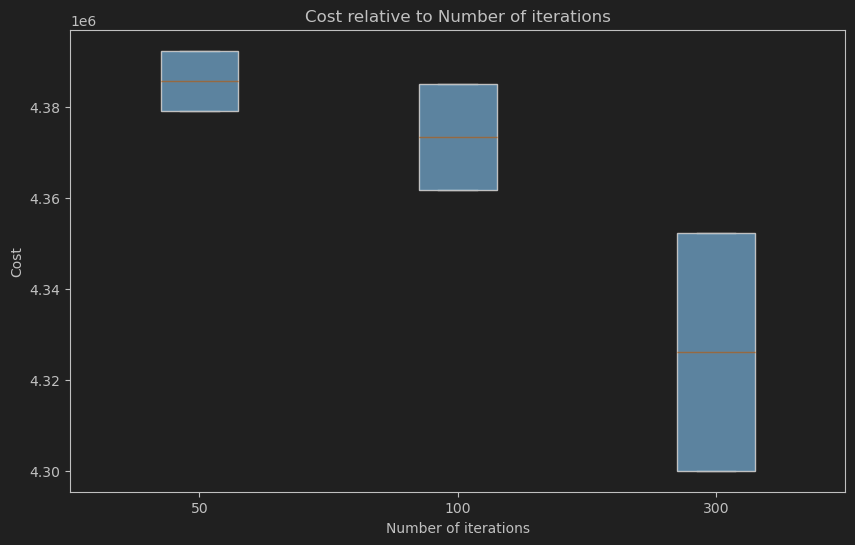
\includegraphics[width=\linewidth]{cost_numit_vnd_med.png}
	\caption{Cost relative to number of iterations on medium tuning instances}
\end{figure}

\begin{figure}[H]
	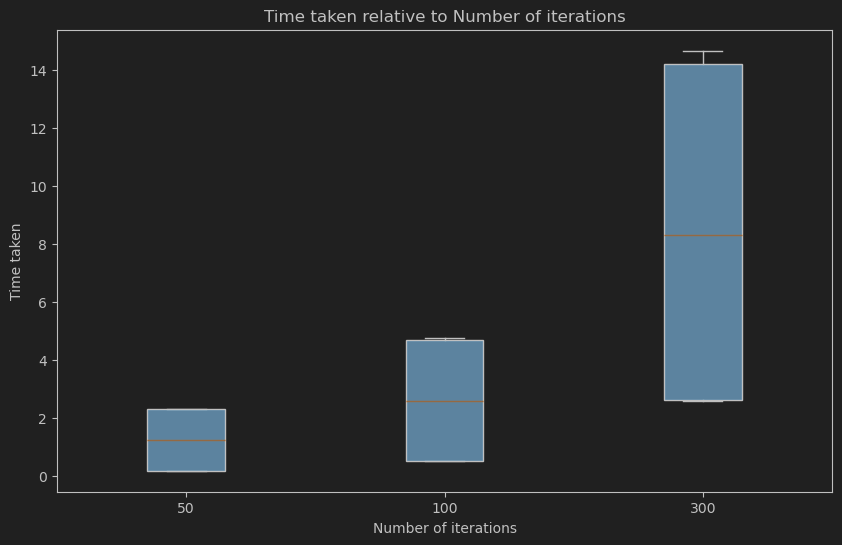
\includegraphics[width=\linewidth]{time_numit_vnd_med.png}
	\caption{Time taken relative to number of iterations on medium tuning instances}
\end{figure}

\paragraph{Step function:}
The step function has a big influence on the solution. The \textit{Random} function is really fast, it doesn't give good solutions so it wasn't used in the tests. While the \textit{Best Improvement} function gives the best result, the time taken to generate the whole neighborhood on larger instances is too large and is beaten in speed and solution cost by the \textit{First Improvement} with a 10 times larger maximum iterations, so the latter was used in most of the tests. The solution cost difference and the time difference can be seen on the following graphs:

\begin{figure}[H]
	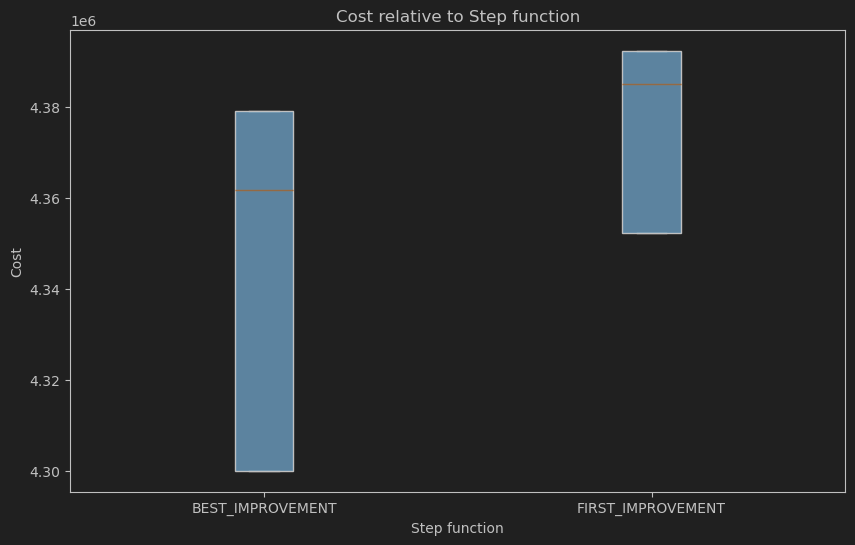
\includegraphics[width=\linewidth]{cost_step_vnd_med.png}
	\caption{Cost relative to step function on medium tuning instances}
\end{figure}

\begin{figure}[H]
	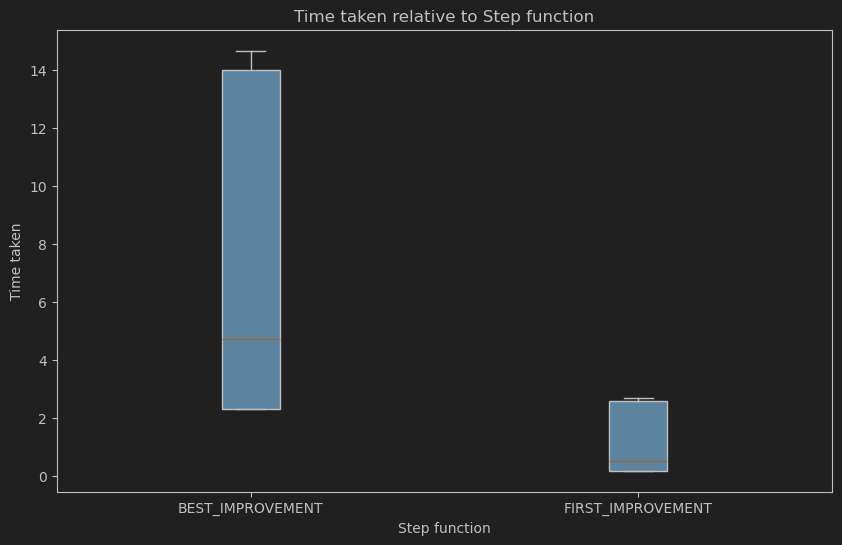
\includegraphics[width=\linewidth]{time_step_vnd_med.png}
	\caption{Time taken relative to step function on medium tuning instances}
\end{figure}


\paragraph{Objective function:}
There are multiple implementations of the cost functions and the 2 most notable are the \textit{cost\_function\_bit} which uses a Fenwick tree to efficiently calculate the cost ($O(E \log V)$, where $E$ is the number of edges) and the cost function which uses delta evaluation using pre calculated prefix sums of weights for the nodes and using only the nodes that have changed ($O(E*diff)$, where $diff$ is the number of changed node). In most cases the second function was used as it performs better in most cases, but the perfomance gains vary based on the machine the experiments were ran on.

\paragraph{Neighborhood order:}
The order of the neighborhood functions also has a big influence on speed, and a lesser influence on cost. The \textit{Swap} neighborhood is the fastes but performs the worst, \textit{Reverse} neigbhborhood performs the second best in both aspects and the \textit{Insert} neigbhborhood is the slowest and give an almost negligeble cost improvement over the \textit{Reverse} neigbhborhood. For larger instances, the first neighborhood in the order must be the \textit{Swap} neighborhood as otherwise it would take too much time. This can be seen on the following graph:
\begin{figure}[H]
	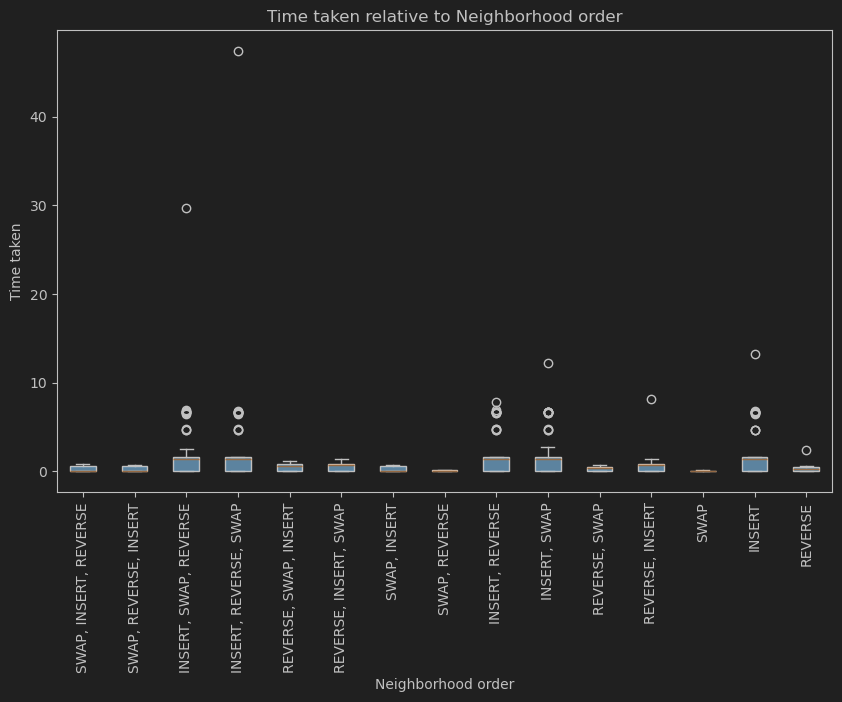
\includegraphics[width=\linewidth]{time_norder_vnd_small.png}
	\caption{Time taken relative to Neighborhood order on small tuning instances}
\end{figure}




\subsection*{Performance}
The tests were ran on a Macbook Pro 16" M2 Pro. The VND algorithm is deterministic in these tests, and that is why the std dev was column left out, the other columns were kept for appearance and to show that it was deterministic.

\subsection*{Small}

\begin{table}[H]
	\centering
 \caption{Results for Small Instances \\($max\_iterations \,{=}\, 250\,, neighborhood\_order \,{=}\, [Swap, Reverse, Insert]$, $step\_function \,{=}\, First\_Improvement$, $Times\, ran \,{=}\, 10$)}
    \hspace*{-1cm}
	\begin{tabular}{lrrrrr}
		\toprule
		\textbf{Item} & \textbf{Avg Time (s)} & \textbf{Avg Cost} & \textbf{Min Cost} & \textbf{Max Cost}  \\
		\midrule
		\texttt{inst\_50\_4\_00002} & 0.3237 & 23982.0 & 23982.0 & 23982.0 \\ 
		\texttt{inst\_50\_4\_00004} & 0.3877 & 6534.0  & 6534.0  & 6534.0  \\ 
		\texttt{inst\_50\_4\_00007} & 0.2896 & 2054.0  & 2054.0  & 2054.0  \\ 
		\texttt{inst\_50\_4\_00005} & 0.3616 & 3580.0  & 3580.0  & 3580.0  \\ 
		\texttt{inst\_50\_4\_00009} & 0.9380 & 1303.0  & 1303.0  & 1303.0  \\ 
		\texttt{inst\_50\_4\_00003} & 0.4459 & 12278.0 & 12278.0 & 12278.0 \\ 
		\texttt{inst\_50\_4\_00006} & 0.2992 & 2959.0  & 2959.0  & 2959.0  \\ 
		\texttt{inst\_50\_4\_00010} & 0.2575 & 857.0   & 857.0   & 857.0   \\ 
		\texttt{inst\_50\_4\_00001} & 1.0881 & 74406.0 & 74406.0 & 74406.0 \\ 
		\texttt{inst\_50\_4\_00008} & 0.1650 & 1405.0  & 1405.0  & 1405.0  \\ 
		\midrule
		\textbf{Summary Statistics} & \textbf{0.4554} & \textbf{12935.8} & - & - \\
		\bottomrule
	\end{tabular}
	\label{tab:performance_metrics_small_vnd}
\end{table}


\subsection*{Medium}
\begin{table}[H]
 	 \centering 
     \caption{Results for Medium Instances \\($max\_iterations \,{=}\, 250\,, neighborhood\_order \,{=}\, [Swap, Reverse, Insert]$, $step\_function \,{=}\, First\_Improvement$, $Times\, ran \,{=}\, 10$)}
     \hspace*{-1cm}
 	 \begin{tabular}{lrrrrr} 
 	 	\toprule 
 	 	\textbf{Item} & \textbf{Avg Time (s)} & \textbf{Avg Cost} & \textbf{Min Cost} & \textbf{Max Cost} \\ 
 	 	\midrule 
 	 	\texttt{inst\_200\_20\_00010} & 0.9009 & 454212.00 & 454212.00 & 454212.00  \\ \texttt{inst\_200\_20\_00009} & 0.6965 & 539627.00 & 539627.00 & 539627.00 \\ \texttt{inst\_200\_20\_00008} & 0.9636 & 700167.00 & 700167.00 & 700167.00 \\  \texttt{inst\_200\_20\_00007} & 1.2543 & 892949.00 & 892949.00 & 892949.00 \\  \texttt{inst\_200\_20\_00006} & 1.1160 & 1198988.00 & 1198988.00 & 1198988.00 \\  \texttt{inst\_200\_20\_00005} & 1.6312 & 1608128.00 & 1608128.00 & 1608128.00 \\  \texttt{inst\_200\_20\_00004} & 2.0465 & 2524537.00 & 2524537.00 & 2524537.00 \\  \texttt{inst\_200\_20\_00003} & 2.0466 & 4308610.00 & 4308610.00 & 4308610.00 \\  \texttt{inst\_200\_20\_00002} & 3.8624 & 8306145.00 & 8306145.00 & 8306145.00 \\  \texttt{inst\_200\_20\_00001} & 5.4359 & 22865269.00 & 22865269.00 & 22865269.00 \\ 
 	 	\midrule 
 	 	\textbf{Summary Statistics} & \textbf{1.9953} & \textbf{4339863.2} & - & - \\ 
 	 	\bottomrule
 	  \end{tabular}
 	  \label{tab:performance_metrics_medium_vnd}
\end{table}

\subsection*{Medium-Large}
\begin{table}[H]
	\centering
	     \caption{Results for Medium-Large Instances \\($max\_iterations \,{=}\, 250\,, neighborhood\_order \,{=}\, [Swap, Reverse, Insert]$, $step\_function \,{=}\, First\_Improvement$, $Times\, ran \,{=}\, 10$)}
    \hspace*{-1cm}

	\begin{tabular}{lrrrrr}
		\toprule
		\textbf{Item} & \textbf{Avg Time (s)} & \textbf{Avg Cost} & \textbf{Min Cost} & \textbf{Max Cost} \\
		\midrule
		\texttt{inst\_500\_40\_00001} & 7.713967 & 40746020.00  & 40746020.00  & 40746020.00  \\
		\texttt{inst\_500\_40\_00010} & 19.30043 & 247021962.00 & 247021962.00 & 247021962.00  \\
		\texttt{inst\_500\_40\_00019} & 26.84756 & 532160524.00 & 532160524.00 & 532160524.00 \\
		\texttt{inst\_500\_40\_00013} & 28.13974 & 333729516.00 & 333729516.00 & 333729516.00 \\
		\texttt{inst\_500\_40\_00007} & 14.91125 & 167816702.00 & 167816702.00 & 167816702.00  \\
		\texttt{inst\_500\_40\_00016} & 25.80133 & 436785606.00 & 436785606.00 & 436785606.00  \\
		\texttt{inst\_500\_40\_00004} & 11.56564 & 94332575.00  & 94332575.00  & 94332575.00  \\
		\midrule
		\textbf{Summary Statistics} & \textbf{19.1828} & \textbf{264656129.29} & - & -  \\
		\bottomrule
	\end{tabular}
	\label{tab:medium_large_performance_metrics_vnd}
\end{table}

\subsection*{Large}
\begin{table}[H]
	\centering
	     \caption{Results for Large Instances \\($max\_iterations \,{=}\, 250\,, neighborhood\_order \,{=}\, [Swap, Reverse, Insert]$, $step\_function \,{=}\, First\_Improvement$, $Times\, ran \,{=}\, 1$)}
    \hspace*{-1cm}
	\begin{tabular}{lrrrrr}
		\toprule
		\textbf{Item} & \textbf{Avg Time (s)} & \textbf{Avg Cost} & \textbf{Min Cost} & \textbf{Max Cost} \\
		\midrule
		\texttt{inst\_1000\_60\_00005} & 48.58142 & 1065061908.00  & 1065061908.00  & 1065061908.00   \\
		\texttt{inst\_1000\_60\_00002} & 126.88115 & 5340070725.00  & 5340070725.00  & 5340070725.00   \\
		\texttt{inst\_1000\_60\_00004} & 47.21685 & 1614136455.00  & 1614136455.00  & 1614136455.00 \\
		\texttt{inst\_1000\_60\_00001} & 275.15735 & 15149609242.00 & 15149609242.00 & 15149609242.00  \\
		\texttt{inst\_1000\_60\_00003} & 98.87615 & 2700741000.00  & 2700741000.00  & 2700741000.00 \\
		\texttt{inst\_1000\_60\_00007} & 32.09443 & 569122169.00   & 569122169.00   & 569122169.00 \\
		\texttt{inst\_1000\_60\_00006} & 41.20420 & 767104436.00   & 767104436.00   & 767104436.00 \\
		\texttt{inst\_1000\_60\_00008} & 34.37336 & 451129061.00   & 451129061.00   & 451129061.00  \\
		\texttt{inst\_1000\_60\_00009} & 23.47634 & 358888563.00   & 358888563.00   & 358888563.00 \\
		\texttt{inst\_1000\_60\_00010} & 23.55307 & 293069393.00   & 293069393.00   & 293069393.00 \\
		\midrule
		\textbf{Summary Statistics} & \textbf{75.14143} & \textbf{2830893295.20}  & - & -  \\
		\bottomrule
	\end{tabular}
	\label{tab:large_performance_metrics_vnd}
\end{table}

\section*{Q7: Greedy Randomized Adaptive Search Procedure(GRASP)}
\subsection*{Algorithm and Adaptations}
In this implementation GRASP uses greedy randomised construction and the VND implementation for local search.  The greedy randomised contruction uses a combination of a greedy approach and randomness to get a solution after which it is refined using VND. The algorithm itself has these parameters that can influence the result: \textbf{max iterations}, \textbf{alpha} (How random is the algorithm), \textbf{neighborhood structures}, \textbf{step function}, \textbf{vnd max iterations}.

\paragraph{Alpha:}
The alpha parameter influences the randomness of the algorithm. It can have a value of 0 to 1 where 0 is purely greedy while 1 being completely random.

\subsection*{Performance Factors:}
The perfomance of the algorithm is influenced by the chosen parameters. Parameters like \textbf{max iterations}, \textbf{neighborhood structures}, \textbf{step function}, \textbf{vnd max iterations} have a very similar influence as in the VND algorithm (as most of the parameters directly influence the VND algorithm which is done as part of GRASP). The only new factor is alpha value.

\paragraph*{Alpha:}
The alpha value doesn't influence the results speed almost at all and influences the cost a little bit. From testing, alpha values around 0.5 are best.

\begin{figure}[H]
	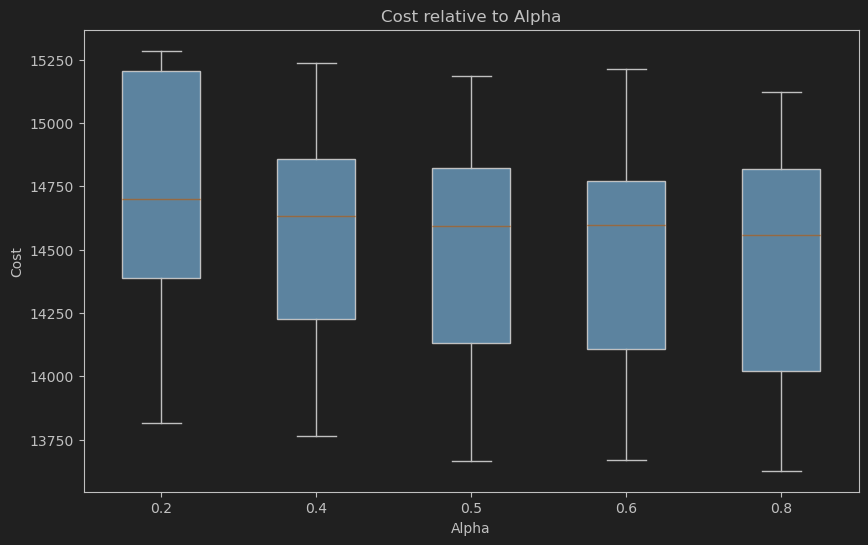
\includegraphics[width=\linewidth]{cost_alpha_grasp_small.png}
	\caption{Cost relative to alpha value on small tuning instances}
\end{figure}

\begin{figure}[H]
	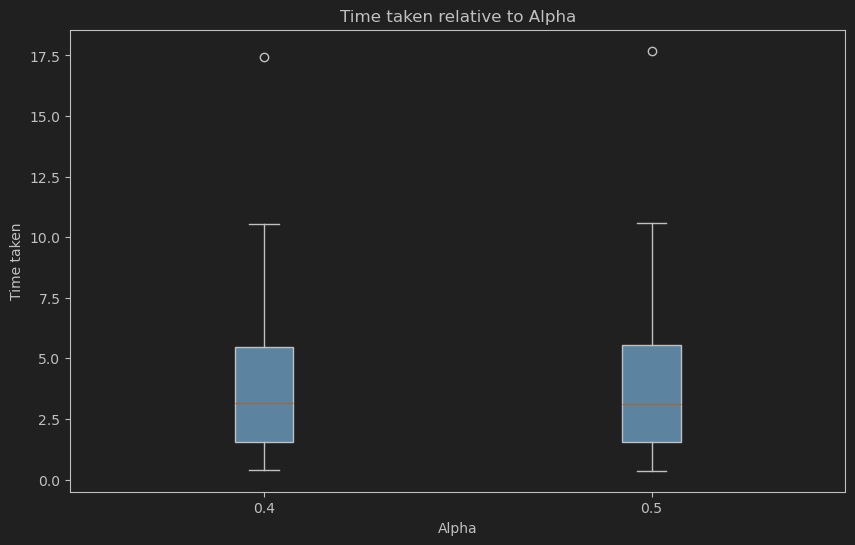
\includegraphics[width=\linewidth]{time_alpha_grasp_med.png}
	\caption{time taken relative to alpha value on medium tuning instances}
\end{figure}


\subsection*{Performance}
The tests were ran on a Macbook Pro 16" M2 Pro. All the test have been ran with the following parameters: 

\subsection*{Small}
\begin{table}[H]
	\centering
  \caption{Results for Small Instances \\($max\_iterations \,{=}\, 25\,, neighborhood\_structures \,{=}\, [Swap, Reverse, Insert]$, $step\_function \,{=}\, First\_Improvement$, $alpha \,{=}\, 0.5$, $vnd\_max\_iterations \,{=}\, 30$, $Times\, ran \,{=}\, 3$)}
    \hspace*{-2cm}
	\begin{tabular}{lrrrrr}
		\toprule
		\textbf{Item} & \textbf{Avg Time (s)} & \textbf{Avg Cost} & \textbf{Min Cost} & \textbf{Max Cost} & \textbf{Std Dev} \\
		\midrule
		\texttt{inst\_50\_4\_00006} & 0.09 & 3645.67 & 3438.0 & 3816.0 & 156.56 \\ 
		\texttt{inst\_50\_4\_00001} & 0.26 & 79158.33 & 77436.0 & 81118.0 & 1512.51 \\ 
		\texttt{inst\_50\_4\_00008} & 0.12 & 2011.0 & 1979.0 & 2063.0 & 37.09 \\ 
		\texttt{inst\_50\_4\_00009} & 0.11 & 1862.67 & 1787.0 & 1976.0 & 81.63 \\ 
		\texttt{inst\_50\_4\_00007} & 0.13 & 2737.0 & 2625.0 & 2881.0 & 106.93 \\ 
		\texttt{inst\_50\_4\_00010} & 0.11 & 1187.67 & 1063.0 & 1272.0 & 89.96 \\ 
		\texttt{inst\_50\_4\_00002} & 0.17 & 27033.33 & 26730.0 & 27628.0 & 420.52 \\ 
		\texttt{inst\_50\_4\_00005} & 0.09 & 4774.33 & 4637.0 & 4895.0 & 105.99 \\ 
		\texttt{inst\_50\_4\_00004} & 0.1 & 8018.67 & 7899.0 & 8152.0 & 103.74 \\ 
		\texttt{inst\_50\_4\_00003} & 0.12 & 13832.33 & 13520.0 & 14066.0 & 229.74 \\ \midrule \textbf{Summary Statistics} & \textbf{0.13} & \textbf{14426.1} & - & - & - \\
		\bottomrule
	\end{tabular}
	\label{tab:performance_metrics_small_grasp}
\end{table}


\subsection*{Medium}
\begin{table}[H]
	\centering 
      \caption{Results for Medium Instances \\($max\_iterations \,{=}\, 25\,, neighborhood\_structures \,{=}\, [Swap, Reverse, Insert]$, $step\_function \,{=}\, First\_Improvement$, $alpha \,{=}\, 0.5$, $vnd\_max\_iterations \,{=}\, 30$, $Times\, ran \,{=}\, 3$)}
    \hspace*{-2cm}
	\begin{tabular}{lrrrrr} 
		\toprule 
		\textbf{Item} & \textbf{Avg Time (s)} & \textbf{Avg Cost} & \textbf{Min Cost} & \textbf{Max Cost} & \textbf{Std Dev} \\
		\midrule 
		\texttt{inst\_200\_20\_00007} & 0.94 & 873815.33 & 860553.0 & 894055.0 & 14539.79 \\ \texttt{inst\_200\_20\_00009} & 0.68 & 514297.67 & 509342.0 & 518202.0 & 3692.68 \\ \texttt{inst\_200\_20\_00008} & 0.73 & 686921.33 & 674443.0 & 695734.0 & 9070.26 \\ \texttt{inst\_200\_20\_00001} & 3.96 & 23018727.0 & 23010528.0 & 23030165.0 & 8337.52 \\ \texttt{inst\_200\_20\_00006} & 0.97 & 1186009.0 & 1179762.0 & 1197072.0 & 7844.51 \\ \texttt{inst\_200\_20\_00003} & 1.73 & 4251857.33 & 4236641.0 & 4264974.0 & 11661.79 \\ \texttt{inst\_200\_20\_00004} & 1.35 & 2464907.67 & 2453273.0 & 2474730.0 & 8853.03 \\ \texttt{inst\_200\_20\_00005} & 1.1 & 1591541.33 & 1586903.0 & 1598403.0 & 4951.09 \\ \texttt{inst\_200\_20\_00002} & 2.48 & 8222953.33 & 8197958.0 & 8263860.0 & 29162.15 \\ \texttt{inst\_200\_20\_00010} & 0.62 & 440797.67 & 435309.0 & 446191.0 & 4443.07 \\ \midrule \textbf{Summary Statistics} & \textbf{1.46} & \textbf{4325182.77} & - & - & - \\
		\bottomrule
	\end{tabular}
	\label{tab:performance_metrics_medium_grasp}
\end{table}


\subsection*{Medium-Large}
\begin{table}[H]
	\centering
      \caption{Results for Medium-Large Instances \\($max\_iterations \,{=}\, 10\,, neighborhood\_structures \,{=}\, [Swap, Reverse, Insert]$, $step\_function \,{=}\, First\_Improvement$, $alpha \,{=}\, 0.5$, $vnd\_max\_iterations \,{=}\, 50$, $Times\, ran \,{=}\, 3$)}
    \hspace*{-2cm}
	\begin{tabular}{lrrrrr}
		\toprule
		\textbf{Item} & \textbf{Avg Time (s)} & \textbf{Avg Cost} & \textbf{Min Cost} & \textbf{Max Cost} & \textbf{Std Dev}\\
		\midrule
		\texttt{inst\_500\_40\_00007} & 13.72 & 166310372.33 & 165867439.0 & 166625627.0 & 322426.88 \\ \texttt{inst\_500\_40\_00001} & 6.07 & 40830970.67 & 40664286.0 & 41026713.0 & 149380.04 \\ \texttt{inst\_500\_40\_00013} & 17.89 & 332086961.67 & 331656754.0 & 332894660.0 & 571534.32 \\ \texttt{inst\_500\_40\_00004} & 9.84 & 93503367.33 & 93157934.0 & 93737576.0 & 249365.07 \\ \texttt{inst\_500\_40\_00016} & 21.62 & 434561356.33 & 433826284.0 & 435492020.0 & 693955.37 \\ \texttt{inst\_500\_40\_00019} & 24.19 & 530075699.33 & 528693872.0 & 531219960.0 & 1044863.18 \\ \texttt{inst\_500\_40\_00010} & 18.06 & 247358297.0 & 247233882.0 & 247525121.0 & 122621.18 \\ \midrule \textbf{Summary Statistics} & \textbf{15.91} & \textbf{263532432.1} & - & - & - \\
		\bottomrule
	\end{tabular}
	\label{tab:medium_large_performance_metrics_grasp}
\end{table}


\subsection*{Large}
\begin{table}[H]
	\centering
      \caption{Results for Large Instances \\($max\_iterations \,{=}\, 10\,, neighborhood\_structures \,{=}\, [Swap, Reverse, Insert]$, $step\_function \,{=}\, First\_Improvement$, $alpha \,{=}\, 0.5$, $vnd\_max\_iterations \,{=}\, 50$, $Times\, ran \,{=}\, 3$)}
    \hspace*{-2cm}
	\begin{tabular}{lrrrrr}
		\toprule
		\textbf{Item} & \textbf{Avg Time (s)} & \textbf{Avg Cost} & \textbf{Min Cost} & \textbf{Max Cost} & \textbf{Std Dev} \\
		\midrule
		\texttt{inst\_1000\_60\_00010} & 20.46 & 292386461.67 & 291941757.0 & 292920610.0 & 404589.03 \\ \texttt{inst\_1000\_60\_00003} & 66.39 & 2705458074.67 & 2704395967.0 & 2706959443.0 & 1091654.63 \\ \texttt{inst\_1000\_60\_00004} & 49.53 & 1615570631.0 & 1613969923.0 & 1616593173.0 & 1146317.9 \\ \texttt{inst\_1000\_60\_00005} & 38.42 & 1062952053.0 & 1059184520.0 & 1066418625.0 & 2960968.53 \\ \texttt{inst\_1000\_60\_00002} & 91.55 & 5330197092.0 & 5324271923.0 & 5333652965.0 & 4209042.2 \\ \texttt{inst\_1000\_60\_00009} & 23.65 & 354315466.0 & 353641813.0 & 354924422.0 & 525617.57 \\ \texttt{inst\_1000\_60\_00007} & 31.48 & 565296811.67 & 563808813.0 & 567536448.0 & 1611941.91 \\ \texttt{inst\_1000\_60\_00001} & 157.72 & 15113519288.67 & 15107419897.0 & 15125357898.0 & 8372452.23 \\ \texttt{inst\_1000\_60\_00006} & 32.78 & 767352749.0 & 766341523.0 & 769276827.0 & 1361121.22 \\ \texttt{inst\_1000\_60\_00008} & 27.94 & 446535007.33 & 446328525.0 & 446639785.0 & 146010.45 \\ \midrule \textbf{Summary Statistics} & \textbf{53.99} & \textbf{2825358363.5} & - & - & - \\
		\bottomrule
	\end{tabular}
	\label{tab:large_performance_metrics_grasp}
\end{table}

\section*{Q8: General Variable Neighborhood Search(GVNS)}
\subsection*{Algorithm and Adaptations}
GVNS combines the VND with random shaking to try to give the VND a chance to escape a local optima. In the implementation, it supports different implementations of VND and it has these parameters:  \textbf{shaking neighborhoods},  \textbf{local search neighborhoods},  \textbf{objective function},  \textbf{maximum number of iterations},  \textbf{vnd step function},  \textbf{vnd max iterations}. The only completely new parameter which was introduced was \textbf{shaking neighborhoods} and it is explained in the next paragraph.

\paragraph{Shaking neighborhoods:}
Similar to neighborhoods, shaking neighborhoods are possible solutions which can be achieved using specific rules from the current solution. The shaking neighborhoods are special as they always provide only one random solution from the counterpart normal neighborhood. These were the implemented ones:
\begin{itemize}
	\item \textbf{Swap neighborhood (n):} It returns a solution which can be found in the swap neighborhood. It also supports the creation of a swap-n neighborhood, which allows all solutions which can be achieved using n swaps from the current solution.
	\item \textbf{Insert neighborhood:} It returns a solution from the insert neighborhood.
	\item \textbf{Reverse neighborhood:} It returns a solution from the reverse neighborhood.
\end{itemize}

\subsection*{Performance factors}
The main new performance factor was the shaking neighborhoods. The number of iterations performed was generaly lower, as the iteration incremented only when a better solution was not found using the pass trough shaking neighborhoods and VND after each of the shakes. 

\paragraph{Shaking neigborhoods:}
The shaking neigborhoods definitely had an influence on the result, mainly with neghborhoods which aren't present in the VND. Those were the swap-n neigborhoods. The neigborhoods had a bigger influence on the resulting cost than on time, which shows that even less iterations with more neigborhoods can improve the results but also extend the time needed for the instance. The impact can be seen on these graphs:

\begin{figure}[H]
	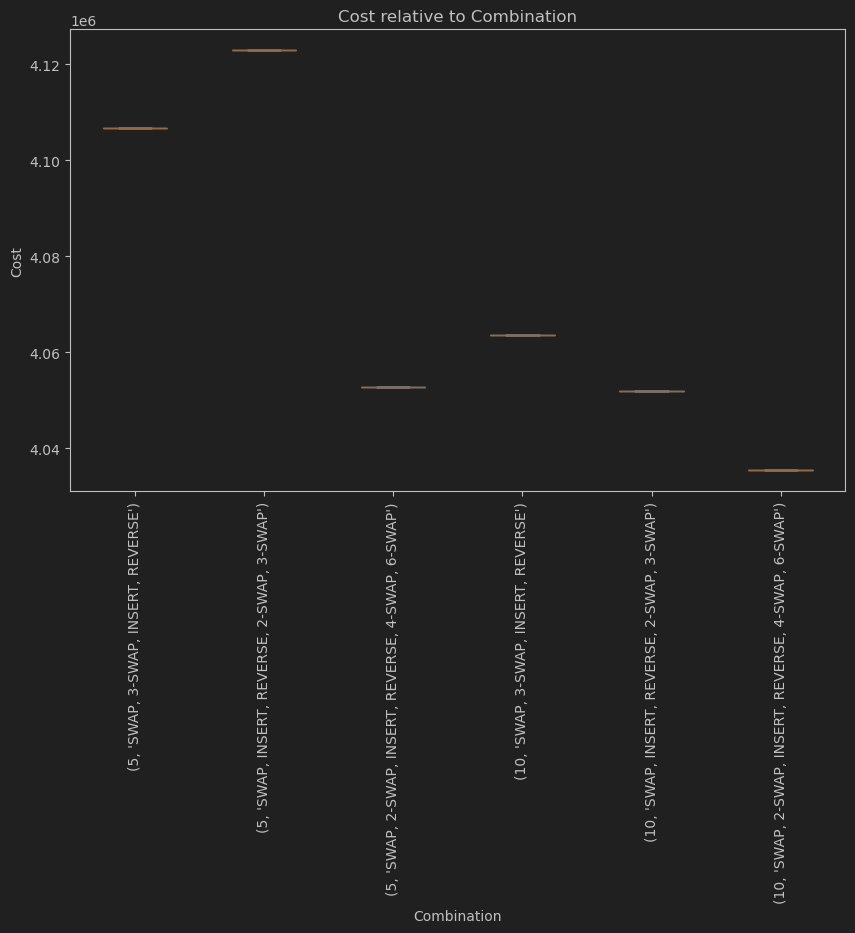
\includegraphics[width=\linewidth]{cost_combination_gvns_med.png}
	\caption{Cost relative to combinations on medium tuning instances}
\end{figure}

\begin{figure}[H]
	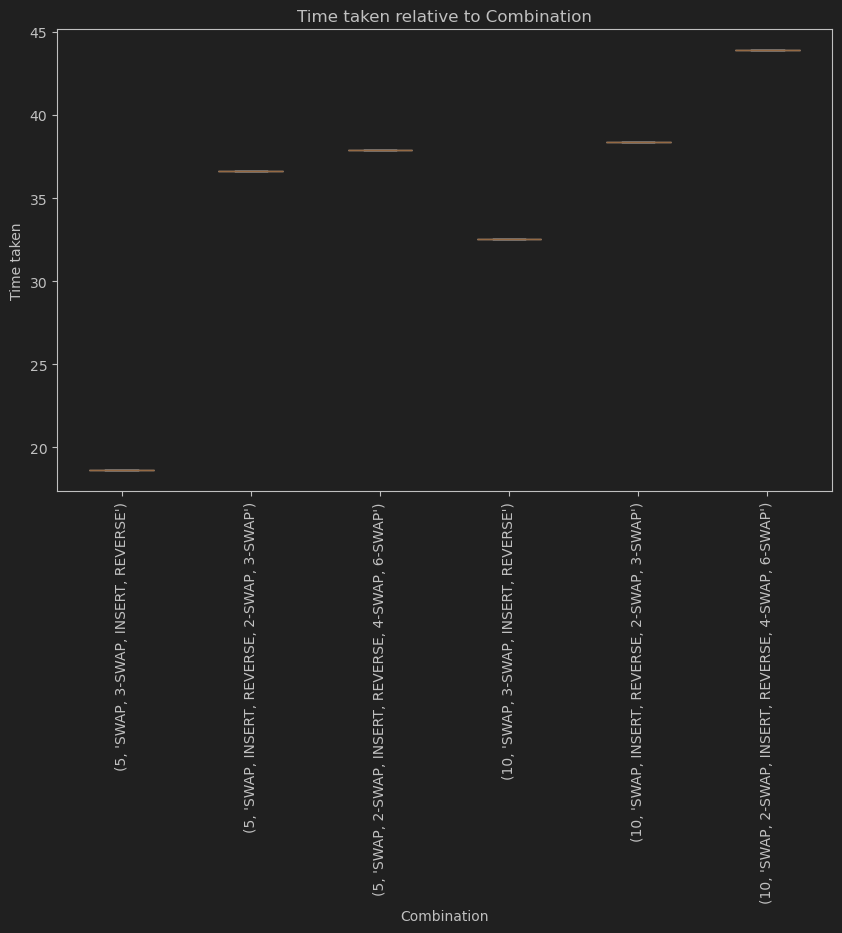
\includegraphics[width=\linewidth]{time_comb_gvns_med.png}
	\caption{Time taken relative to combinations on medium tuning instances}
\end{figure}

\subsection*{Performance}
The tests were ran on a Macbook Pro 16" M2 Pro.

\subsection*{Small}
\begin{table}[H]
	\centering
   \caption{Results for Small Instances \\($max\_iterations \,{=}\, 3\,, neighborhood\_structures \,{=}\, [Swap, Reverse, Insert]$, $step\_function \,{=}\, First\_Improvement$, $neighborhood\_shake\_order \,{=}\, [Swap, Swap-3, Insert, Reverse]$, $vnd\_max\_iterations \,{=}\, 50$, $Times\, ran \,{=}\, 3$)}
    \hspace*{-1cm}
	\begin{tabular}{lrrrrr}
		\toprule
		\textbf{Item} & \textbf{Avg Time (s)} & \textbf{Avg Cost} & \textbf{Min Cost} & \textbf{Max Cost} & \textbf{Std Dev} \\
		\midrule
		\texttt{inst\_50\_4\_00006} & 0.04 & 3210.0 & 3134.0 & 3253.0 & 53.89 \\ \texttt{inst\_50\_4\_00001} & 0.11 & 76150.0 & 75438.0 & 77430.0 & 907.0 \\ \texttt{inst\_50\_4\_00008} & 0.03 & 1585.33 & 1414.0 & 1736.0 & 132.27 \\ \texttt{inst\_50\_4\_00009} & 0.04 & 1506.0 & 1367.0 & 1686.0 & 133.42 \\ \texttt{inst\_50\_4\_00007} & 0.05 & 2184.33 & 2131.0 & 2283.0 & 69.84 \\ \texttt{inst\_50\_4\_00010} & 0.03 & 1003.67 & 906.0 & 1077.0 & 71.9 \\ \texttt{inst\_50\_4\_00002} & 0.1 & 25192.0 & 24033.0 & 26068.0 & 854.55 \\ \texttt{inst\_50\_4\_00005} & 0.04 & 4078.0 & 3857.0 & 4520.0 & 312.54 \\ \texttt{inst\_50\_4\_00004} & 0.02 & 7152.33 & 6764.0 & 7404.0 & 278.58 \\ \texttt{inst\_50\_4\_00003} & 0.05 & 13243.67 & 12504.0 & 14237.0 & 729.88 \\ \midrule \textbf{Summary Statistics} & \textbf{0.05} & \textbf{13530.53} & - & - & - \\
		\bottomrule
	\end{tabular}
	\label{tab:performance_metrics_small_gvns}
\end{table}


\subsection*{Medium}
\begin{table}[H]
	\centering 
	   \caption{Results for Medium Instances \\($max\_iterations \,{=}\, 3\,, neighborhood\_structures \,{=}\, [Swap, Reverse, Insert]$, $step\_function \,{=}\, First\_Improvement$, $neighborhood\_shake\_order \,{=}\, [Swap, Swap-3, Insert, Reverse]$, $vnd\_max\_iterations \,{=}\, 50$, $Times\, ran \,{=}\, 3$)}
        \hspace*{-2cm}
	\begin{tabular}{lrrrrr} 
		\toprule 
		\textbf{Item} & \textbf{Avg Time (s)} & \textbf{Avg Cost} & \textbf{Min Cost} & \textbf{Max Cost} & \textbf{Std Dev} \\
		\midrule 
		\texttt{inst\_200\_20\_00007} & 0.6 & 842506.67 & 829973.0 & 866402.0 & 16903.33 \\ \texttt{inst\_200\_20\_00009} & 0.68 & 489406.33 & 467318.0 & 509942.0 & 17435.78 \\ \texttt{inst\_200\_20\_00008} & 0.47 & 662052.0 & 639147.0 & 679630.0 & 16950.93 \\ \texttt{inst\_200\_20\_00001} & 2.66 & 22507012.67 & 22490490.0 & 22528583.0 & 15955.74 \\ \texttt{inst\_200\_20\_00006} & 1.0 & 1115826.0 & 1088608.0 & 1138416.0 & 20595.68 \\ \texttt{inst\_200\_20\_00003} & 1.03 & 4195880.67 & 4111869.0 & 4278554.0 & 68055.45 \\ \texttt{inst\_200\_20\_00004} & 1.78 & 2384060.67 & 2356315.0 & 2407178.0 & 21021.06 \\ \texttt{inst\_200\_20\_00005} & 1.17 & 1493774.0 & 1479795.0 & 1504700.0 & 10394.08 \\ \texttt{inst\_200\_20\_00002} & 2.55 & 8063316.67 & 7987601.0 & 8173461.0 & 79686.82 \\ \texttt{inst\_200\_20\_00010} & 0.61 & 410307.67 & 397507.0 & 420505.0 & 9567.65 \\ \midrule \textbf{Summary Statistics} & \textbf{1.26} & \textbf{4216414.33} & - & - & - \\
		\bottomrule
	\end{tabular}
	\label{tab:performance_metrics_medium_gvns}
\end{table}


\subsection*{Medium-Large}
\begin{table}[H]
	\centering
	   \caption{Results for Medium-Large Instances \\($max\_iterations \,{=}\, 3\,, neighborhood\_structures \,{=}\, [Swap, Reverse, Insert]$, $step\_function \,{=}\, First\_Improvement$, $neighborhood\_shake\_order \,{=}\, [Swap, Swap-3, Insert, Reverse]$, $vnd\_max\_iterations \,{=}\, 50$, $Times\, ran \,{=}\, 3$)}
        \hspace*{-2cm}
	\begin{tabular}{lrrrrr}
		\toprule
		\textbf{Item} & \textbf{Avg Time (s)} & \textbf{Avg Cost} & \textbf{Min Cost} & \textbf{Max Cost} & \textbf{Std Dev}\\
		\midrule
		\texttt{inst\_500\_40\_00007} & 18.55 & 164145155.0 & 162717327.0 & 166669118.0 & 1789841.14 \\ \texttt{inst\_500\_40\_00001} & 3.6 & 40253855.0 & 40070596.0 & 40448589.0 & 154528.17 \\ \texttt{inst\_500\_40\_00013} & 12.47 & 331289568.67 & 329174260.0 & 332429864.0 & 1497270.32 \\ \texttt{inst\_500\_40\_00004} & 14.64 & 92149210.33 & 91092025.0 & 92717383.0 & 748241.14 \\ \texttt{inst\_500\_40\_00016} & 18.52 & 432176726.0 & 429529634.0 & 435550888.0 & 2511353.95 \\ \texttt{inst\_500\_40\_00019} & 43.8 & 524163697.0 & 521723283.0 & 525465670.0 & 1726924.25 \\ \texttt{inst\_500\_40\_00010} & 10.63 & 244826397.67 & 243127940.0 & 246795124.0 & 1509269.91 \\ \midrule \textbf{Summary Statistics} & \textbf{17.46} & \textbf{261286372.81} & - & - & - \\
		\bottomrule
	\end{tabular}
	\label{tab:medium_large_performance_metrics_gvns}
\end{table}


\subsection*{Large}
\begin{table}[H]
	\centering
	   \caption{Results for Large Instances \\($max\_iterations \,{=}\, 3\,, neighborhood\_structures \,{=}\, [Swap, Reverse, Insert]$, $step\_function \,{=}\, First\_Improvement$, $neighborhood\_shake\_order \,{=}\, [Swap, Swap-3, Insert, Reverse]$, $vnd\_max\_iterations \,{=}\, 50$, $Times\, ran \,{=}\, 3$)}
        \hspace*{-2cm}
	\begin{tabular}{lrrrrr}
		\toprule
		\textbf{Item} & \textbf{Avg Time (s)} & \textbf{Avg Cost} & \textbf{Min Cost} & \textbf{Max Cost} & \textbf{Std Dev} \\
		\midrule
		\texttt{inst\_1000\_60\_00010} & 12.28 & 290236069.67 & 289196499.0 & 291399836.0 & 903785.34 \\ \texttt{inst\_1000\_60\_00003} & 34.04 & 2690400621.67 & 2680682212.0 & 2697728029.0 & 7161361.06 \\ \texttt{inst\_1000\_60\_00004} & 41.07 & 1602586794.0 & 1598857305.0 & 1608810749.0 & 4429787.98 \\ \texttt{inst\_1000\_60\_00005} & 50.41 & 1057347341.67 & 1053530753.0 & 1060451784.0 & 2870021.12 \\ \texttt{inst\_1000\_60\_00002} & 160.58 & 5312821449.0 & 5298377503.0 & 5326339581.0 & 11434226.4 \\ \texttt{inst\_1000\_60\_00009} & 17.14 & 356347833.33 & 354439227.0 & 357695882.0 & 1387352.18 \\ \texttt{inst\_1000\_60\_00007} & 32.33 & 562712547.67 & 562109354.0 & 563754014.0 & 739499.3 \\ \texttt{inst\_1000\_60\_00001} & 283.16 & 15084967364.0 & 15071720618.0 & 15096689209.0 & 10250256.14 \\ \texttt{inst\_1000\_60\_00006} & 26.24 & 761452544.67 & 760707897.0 & 762766833.0 & 932084.48 \\ \texttt{inst\_1000\_60\_00008} & 14.15 & 448442266.33 & 446978701.0 & 450526114.0 & 1513185.91 \\ \midrule \textbf{Summary Statistics} & \textbf{67.14} & \textbf{2816731483.2} & - & - & - \\
		\bottomrule
	\end{tabular}
	\label{tab:large_performance_metrics_gvns}
\end{table}

\section*{Q9: Delta Evaluation}
The current cost evaluation algorithm is efficient, operating with a complexity of $O(E \log V)$, where $E$ is the number of edges in the graph and $V$ the length of the permutation. This efficiency stems from using a Fenwick tree as data structure to compute the cost. However, there is room for improvement using delta evaluation, which focuses on incremental updates rather than recalculating the cost from scratch. In particular, delta-evaluation can be employed during the cost calculation step of the algorithm. Specifically, when transitioning from one solution to another during a Variable Neighborhood Descent, only the cost contributions from nodes that have changed positions are recalculated.

\paragraph{Delta Evaluation for Cost Computation:} Steps Using Delta-Evaluation:
\begin{itemize}
    \item Identifying Changed Nodes: The algorithm tracks which nodes (denoted as diff) have changed their position in the solution
    \item Updating Cost Incrementally: Instead of recalculating the total cost by considering all edges, the algorithm recalculates only the edges connected to the changed nodes.
\end{itemize}
This reduces the computational effort significantly, especially when the number of changed nodes (diff) is small.

Thus delta-evaluation results in better performance because it avoids redundant calculations for parts of the solution that remain unchanged. Indeed, many combinatorial optimization problems have solutions in the search space that often differ by only a few changes because the neighborhood structures often make small changes (e.g., swapping two nodes). Without delta-evaluation, the cost computation would unnecessarily recompute all edges in the graph.

\paragraph{Asymptotic Runtime}:
As said without Delta-Evaluation the complexity is $O(E \log V)$. With Delta-Evaluation the complexity becomes $O(\text{diff}  \times V\times maxdeg(V))$, which can be approximated as $O(\text{diff} \times E)$. For small values of diff, this is substantially faster. In practice, diff is often a small fraction of $V$, making the delta-evaluation approach faster for most steps.

\paragraph{Other Elements That Could Benefit from Delta-Evaluation}
Another area that could benefit from a form of delta-evaluation could be feasibility checks. Since feasibility constraints depend on node positions, a form of delta-evaluation could focus only on the nodes that have changed. This would reduce the complexity of verifying constraints across the entire solution.

\paragraph{Preprocessing}
The algorithm precomputes the sum of the weight of all edges that connect to U nodes with value less than the current index in the array when the graph is created which allows it to reduce the computations later on. Also, both algorithms have a simple form of caching which allows them to reuse the cost of the solution if it has already been calculated. This is especially useful in the VND algorithm where the same solution is evaluated multiple times.

\section*{Q10: Tuning}
The results of the tunings are showed in the section corresponding to each algorithm

\section*{Q11: Experiments comparison}
The results of each experiment are shown in the section corresponding to each algorithm. For completeness, we add some plots summarizing some results.

\begin{figure}[H]
	\includegraphics[width=\linewidth]{cost_constr.png}
	\caption{Cost of Deterministic vs Randomized Heuristic Solutions}
\end{figure}

\begin{figure}[H]
	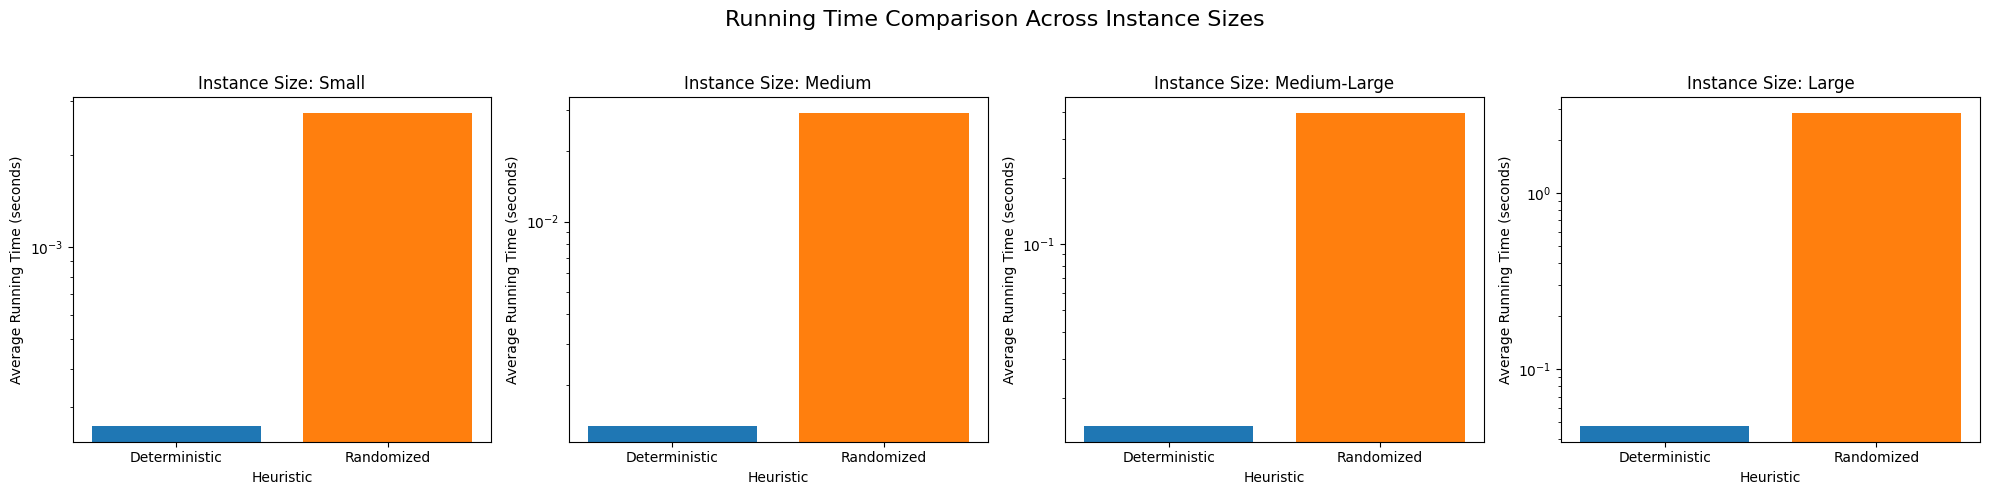
\includegraphics[width=\linewidth]{time_constr.png}
	\caption{Time of Deterministic vs Randomized Heuristic Solutions}
\end{figure}

\begin{figure}[H]
	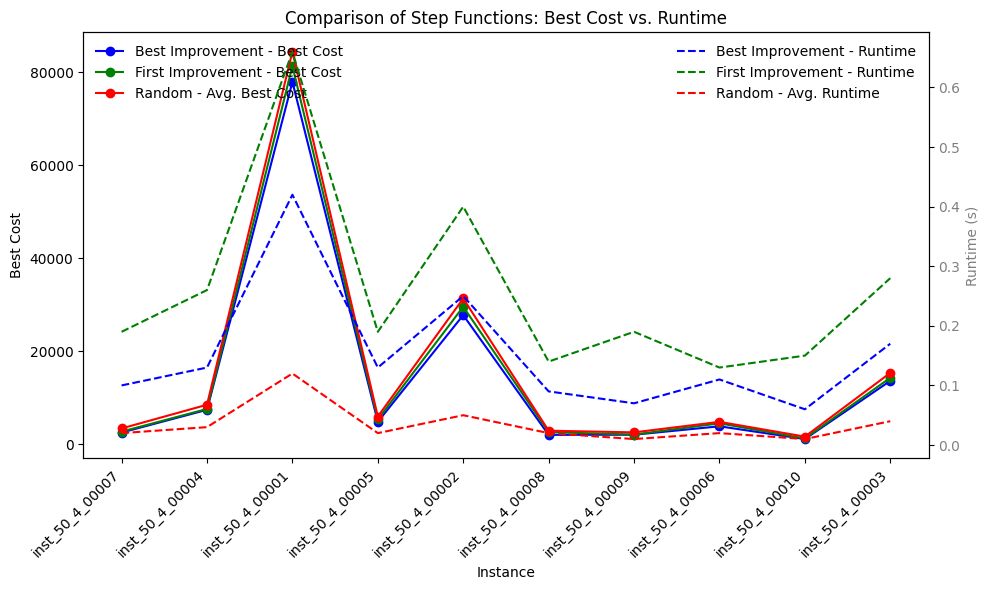
\includegraphics[width=\linewidth]{local_search_swap.png}
	\caption{Time and Cost of Local Search for Small Instances with Different Cost Functions and Swap Neighborhood}
\end{figure}

\begin{figure}[H]
	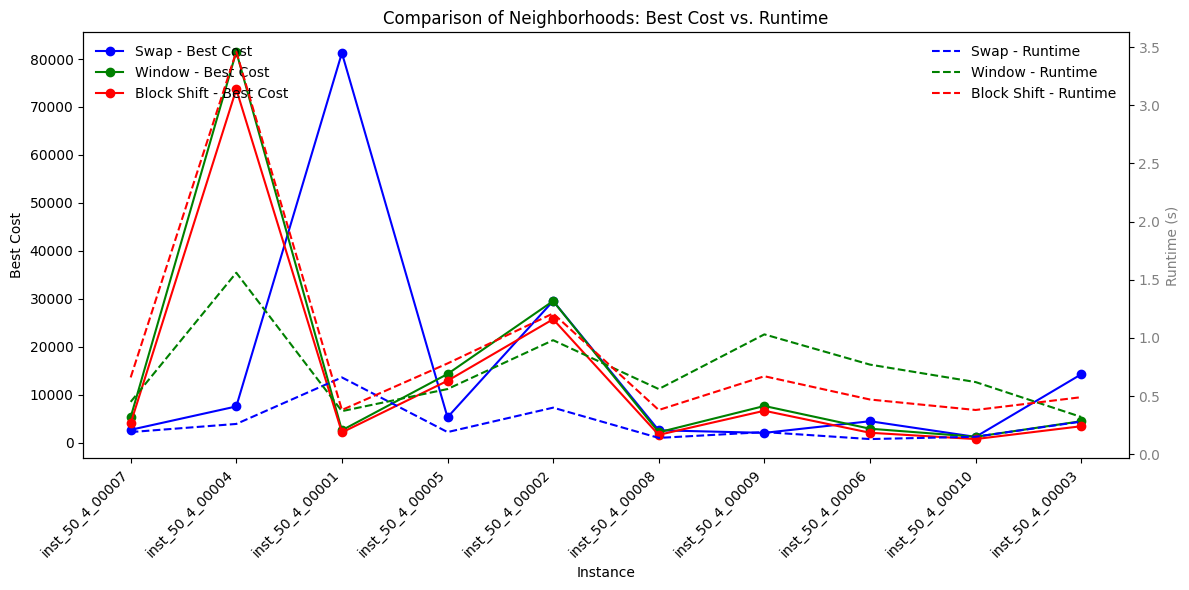
\includegraphics[width=\linewidth]{ls_n.png}
	\caption{Time and Cost of Local Search for Small Instances with Different Neighborhoods and First Improvement}
\end{figure}

\begin{figure}[H]
	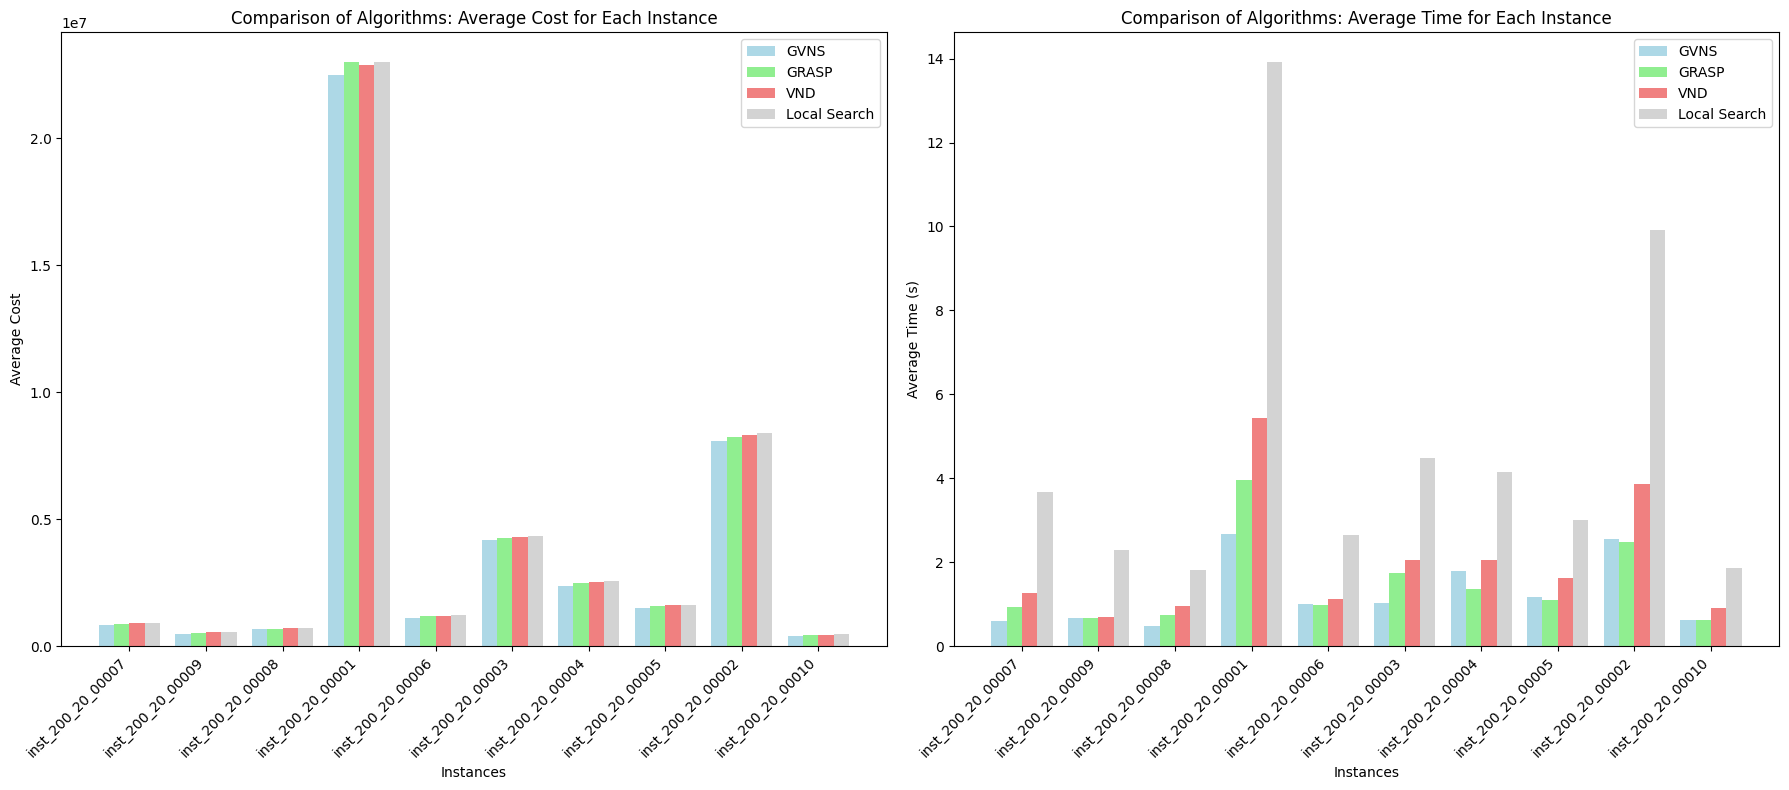
\includegraphics[width=\linewidth]{algo_comp.png}
	\caption{Time and Cost Comparison of Different Optimization Strategies for Medium Instances}
\end{figure}

\end{document}
